\documentclass[12pt]{article}
\usepackage[romanian]{babel}
\usepackage{indentfirst}
\usepackage{amsmath, amssymb, amsfonts, graphicx}
\usepackage{blindtext}
\usepackage{hyperref}
\usepackage{pgfplots}
\usepackage{subcaption}
\usepackage{makecell}
\pgfplotsset{compat=1.17}

\newcommand{\HRule}[1]{\rule{\linewidth}{#1}}


\begin{document}
\begin{titlepage}
    \centering

	\includegraphics[width=0.5\textwidth]{images/logo2.png} \\[70pt]

    \HRule{0.5pt} \\
    \LARGE \textbf{\uppercase{Eliminarea zgomotului si restituirea imaginii în procesarea imaginilor digitale}}
    \HRule{2pt} \\ [0.5cm]
    \normalsize {Ianuarie 2024} \vspace*{5\baselineskip} \\[110pt]

    \begin{flushleft}
        \centering

        \textbf{Autori:} \\
        Victor David \\
        Laurențiu-Vasile Crețu \\
        Robert-Alexandru Sorete \\ 
        Nicoleta-Anastasia Dinoiu
    \end{flushleft}
    
\end{titlepage}
\newpage

\tableofcontents
\newpage

%%%%%%%%%%%%%%% Introducere

\section{Introducere}
\label{sec:intro}
Într-o lume din ce în ce mai digitală, imaginile digitale joacă un rol important în aplicațiile de zi cu zi, cum ar fi camerele digitale, imagistica prin rezonanță magnetică, televiziunea prin satelit, precum și în domeniile de cercetare și tehnologie, cum ar fi sistemul de informații geografice. În general, seturile de date colectate de senzorii de imagine sunt contaminate de zgomot. 

Instrumente imperfecte, probleme cu procesul de achiziție a datelor, fenomenele naturale care interferează, toate acestea pot corupe datele de interes. Din acest motiv, reducerea zgomotului devine o etapă fundamentală în procesul de analiză a imaginilor, marcând primul pas ce trebuie efectuat înainte de analiza concisă a imaginilor. 

Zgomotul poate fi adăugat și în procesul de îmbătrânire a imaginilor, manifestându-se prin fenomenele de îngălbenire sau crăpare a imaginilor, cât și prin erori de capturare a imaginii manifestate prin motion blur. Astfel, metodele de eliminare a zgomotului sunt necesare pentru a preveni aceste tipuri de corupție din imaginile digitale.

În această lucrare sunt expuse principalele metode de reducere a zgomotului în imagini, dar și implementarea unor algoritmi destinați recuperării și recondiționării imaginilor în urma fenomenelor de motion blur și de îmbătrânire a imaginilor.

\subsection{Contextul și Importanța Eliminării Zgomotului din Imagini}

\indent Una dintre provocările fundamentale în domeniul procesării imaginilor și viziunii calculatoarelor este reprezentată de eliminarea zgomotului din imagini, unde obiectivul principal este de a estima imaginea originală prin suprimarea zgomotului dintr-o versiune a acesteia contaminată de zgomot. Eliminarea zgomotului joacă un rol important într-o gamă largă de aplicații, cum ar fi restaurarea imaginilor, segmentarea imaginilor și clasificarea imaginilor, unde obținerea conținutului original al imaginii este crucială.

\indent Scopul este de a diminua zgomotul în imagini naturale, minimizând pierderea caracteristicilor originale și îmbunătățind raportul semnal-zgomot (SNR). Principalele provocări pentru reducerea zgomotului în imagini sunt următoarele: zonele plate ar trebui să fie netede, marginile ar trebui protejate fără a fi estompate, texturile ar trebui să fie păstrate, iar noi artefacte nu ar trebui să fie generate.

\begin{figure}[h]
    \centering
    \includegraphics[width=1\textwidth]{images/img1.png}
    \caption{Exemplu de înlăturare a zgomotului cu filtrul Wiener}
    \label{fig:img1}
    \vspace{10pt}
\end{figure}

\subsection{Istoric}
\indent Eliminare zgomotului din imagini are o istorie bogată, începând cu dezvoltarea teoriei filtrării Wiener-Kolmogorov în anii 1940. Această teorie a pus bazele proiectării filtrelor pentru procesele gaussiene staționare. De-a lungul deceniilor, au fost aduse contribuții semnificative de către Peter Swerling, Ruslan Stratonovich și Rudolf Kalman, conducând la aplicații în radar, sateliți și filtrare adaptivă.

\indent În anii 1970, atenția s-a îndreptat către semnale bidimensionale precum imagini digitale. Suprimarea zgomotului din imagini a fost explorată inițial de Nasser Nahi și Ali Habibi, în timp ce filtrarea Kalman a fost extinsă la 2D. Cu toate acestea, limitările practice au împiedicat utilizarea pe scară largă până în anii 1980, până când s-a ajuns la un avans tehnologic necesar. Lucrarea lui Jong-Sen Lee din anii 1980 a implementat filtrarea Kalman 2D pentru îmbunătățirea imaginilor/filtrarea zgomotului, deschizând calea pentru aplicații în inginerie. La sfârșitul anilor 1980 a apărut teoria undinelor (Wavelet Transform), ce a devenit o unealtă populară pentru sarcini de procesare a imaginilor, între anii 1990 și începutul anilor 2000 având loc o creștere a algoritmilor de eliminare a zgomotului bazați pe wavelets.
\newpage


%%%%%%%%%%%%%%% Zgomotul

\section{Zgomotul imaginilor digitale}
\label{sec:zgomot_imagini_digitale}
Zgomotul în imagini digitale reprezintă variațiile nedorite ale intensității pixelilor care sunt introduse în imagine în timpul procesului de capturare, stocare sau transmitere a acesteia. Aceste variații pot fi cauzate de factori precum perturbările în procesul de capturare a imaginii, interferențe electromagnetice, erori de senzori, sau alte influențe externe și interne care conduc la modificări ale intensității pixelilor in mod aleator sau periodic. \\


\subsection{Conceptul de reducere al zgomotului}
Reducerea zgomotului din imagini îmbunătățește calitatea imaginilor printr-o serie de operații, în timp ce încearcă să păstreze informațiile originale și să îndepărteze informațiile redundante din semnal. Într-o aplicație practică este crucială studierea acestui algoritm, deoarece în procesarea de imagini medicale, orice eroare minimale poate afecta diagnoza unui doctor sau poate pune viața unui pacient în pericol. \\

\subsection{Zgomotul Aditiv si Multiplicativ}
Zgomotul aditiv este reprezentat în felul următor:
\begin{equation}
w(x, y) = s(x, y) + n(x, y),
\end{equation}
unde ${s(x, y)}$ este imaginea originală și ${n(x, y)}$ denotă zgomotul introdus pentru a produce imaginea coruptă ${w(x, y)}$ la locația pixelului ${(x, y)}$. Câteva exemple de zgomot aditiv sunt: zgomotul Gaussian, Uniform, Poisson, Impulsiv (Sare și Piper). \\
 
Zgomotul multiplicativ poate fi definit de următoarea formulă:
\begin{equation}
W(x, y) = s(x, y) * n(x, y),
\end{equation}
unde ${s(x, y)}$ și ${n(x, y)}$ sunt aceleași ca mai sus. Unele dintre cele mai cunoscute tipuri de zgomote multiplicative sunt zgomotul Speckle și cel Exponențial. \\


\subsection{Zgomotul Gaussian}
Zgomotul Gaussian este uniform distribuit asupra semnalului. Acest lucru înseamnă că fiecare pixel din imagine este suma dintre valoarea reală a pixelului și a unei valori aleatoare de zgomot a distribuției Gaussiene. Așa cum indică și numele, acest tip de zgomot urmează o distribuție Gaussiană.

\begin{equation}
F(g) = \frac{\frac{1}{\sqrt{2\pi\sigma^2}}  e^{-(g-m)^2}}{2\sigma^2},
\end{equation}
unde ${g}$ reprezintă nivelul de gri, ${m}$ este media sau valoarea medie a funcției, iar ${c}$ este deviația standard a zgomotului. În mod grafic, este reprezentat ca o curbă sub forma unui clopot: \\

\begin{figure}[h]
  \centering
  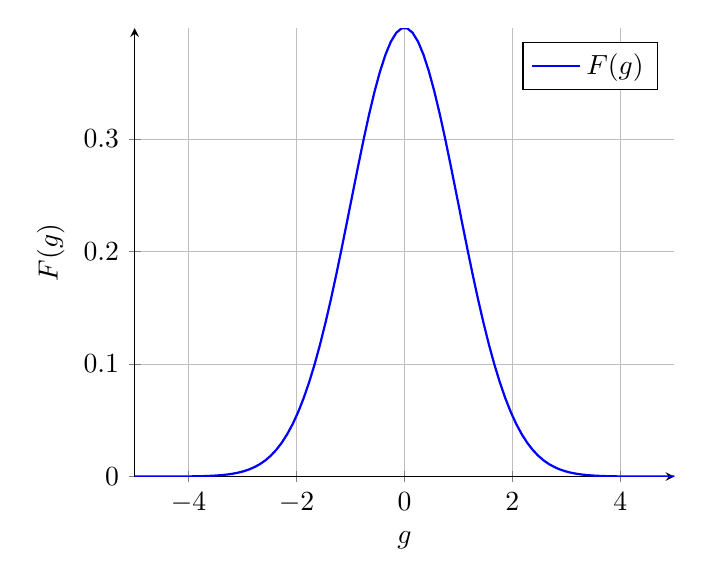
\begin{tikzpicture}
    \begin{axis}[
      xlabel=$g$,
      ylabel=$F(g)$,
      domain=-5:5,
      samples=100,
      axis lines=left,
      grid=both,
      legend pos=north east,
    ]
      \newcommand{\mean}{0}
      \newcommand{\stddev}{1}
      \addplot[blue, thick] {1/(sqrt(2*pi*\stddev^2)) * exp(-(x-\mean)^2/(2*\stddev^2))};
      \addlegendentry{$F(g)$}
    \end{axis}
  \end{tikzpicture}
  \caption{Distribuția Gaussiana}
  \label{fig:gaussian}
\end{figure}


\subsection{Zgomotul Speckle}
Zgomotul Speckle este considerat ca fiind un zgomot multiplicativ. Acesta este un zgomot granular care degradează calitatea imaginilor obținute de sistemele de imagistică coerentă, cum ar fi lasere, radarele active sau sisteme radar cu diafragmă sintetică (SAR). \\
\indent Din cauza fluctuațiilor aleatorii în semnalul de întoarcere al radarului, apare zgomotul de tip speckle, ce poate fi observat prin nivelul crescut de gri al imaginii. Zgomotul Speckle îngreunează interpretarea imaginilor SAR cauzate în principal de procesarea coerentă a semnalelor retrodifuzate (backscatter) de la mai multe ținte distribuite.

Zgomotul de tip speckle urmează o distribuție gamma, care este caracterizată de funcția de densitate de probabilitate:

\begin{equation}
F(g) = \frac{g^{\alpha-1}}{(\alpha-1)! \alpha^{\alpha}} e^{\frac{-g}{\alpha}},
\end{equation}
unde varianța este ${\sigma^2}$ și ${g}$ reprezintă nivelul de gri. \\

\begin{figure}[h]
  \centering
  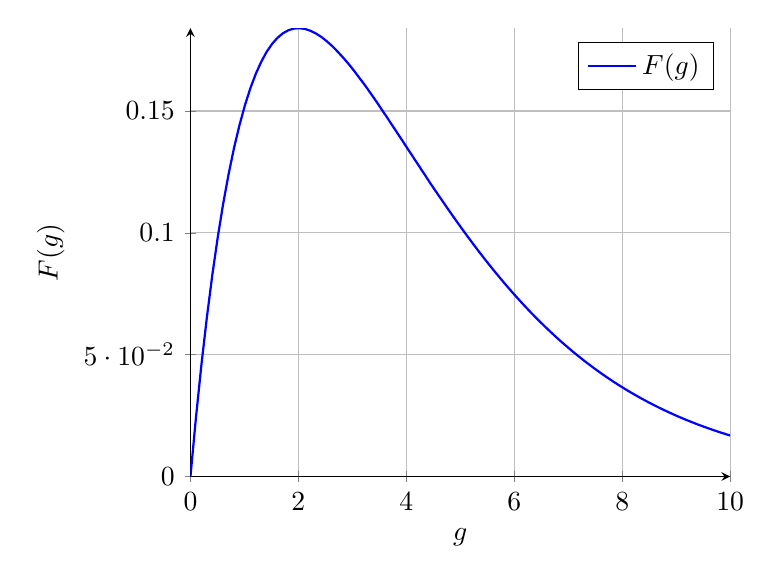
\begin{tikzpicture}
    \begin{axis}[
      xlabel=$g$,
      ylabel=$F(g)$,
      domain=0:10,
      samples=100,
      axis lines=left,
      grid=both,
      legend pos=north east,
    ]
      \newcommand{\alphaValue}{2}
      \addplot[blue, thick] {x^(\alphaValue-1) / (\alphaValue-1)! / \alphaValue^\alphaValue * exp(-x/\alphaValue)};
      \addlegendentry{$F(g)$}
    \end{axis}
  \end{tikzpicture}
  \caption{Distribuția Gamma}
  \label{fig:gamma_distribution}
\end{figure}



\subsection{Zgomotul Impulsiv}
Zgomotul Impulsiv este adesea numit sare-și-piper sau zgomot de impulsuri. O imagine ce conține acest tip de zgomot va avea pixeli închiși in zonele deschise si pixeli deschiși la culoare in regiunile întunecate. Poate fi cauzat de pixeli morți, erori de conversie sau erori de transmisie a datelor. 
\newpage

\subsection{Analiza Histogramelor pentru Diverse Tipuri de Zgomot}

\begin{figure}[h!]
    \begin{subfigure}{0.49\textwidth}
        \centering
        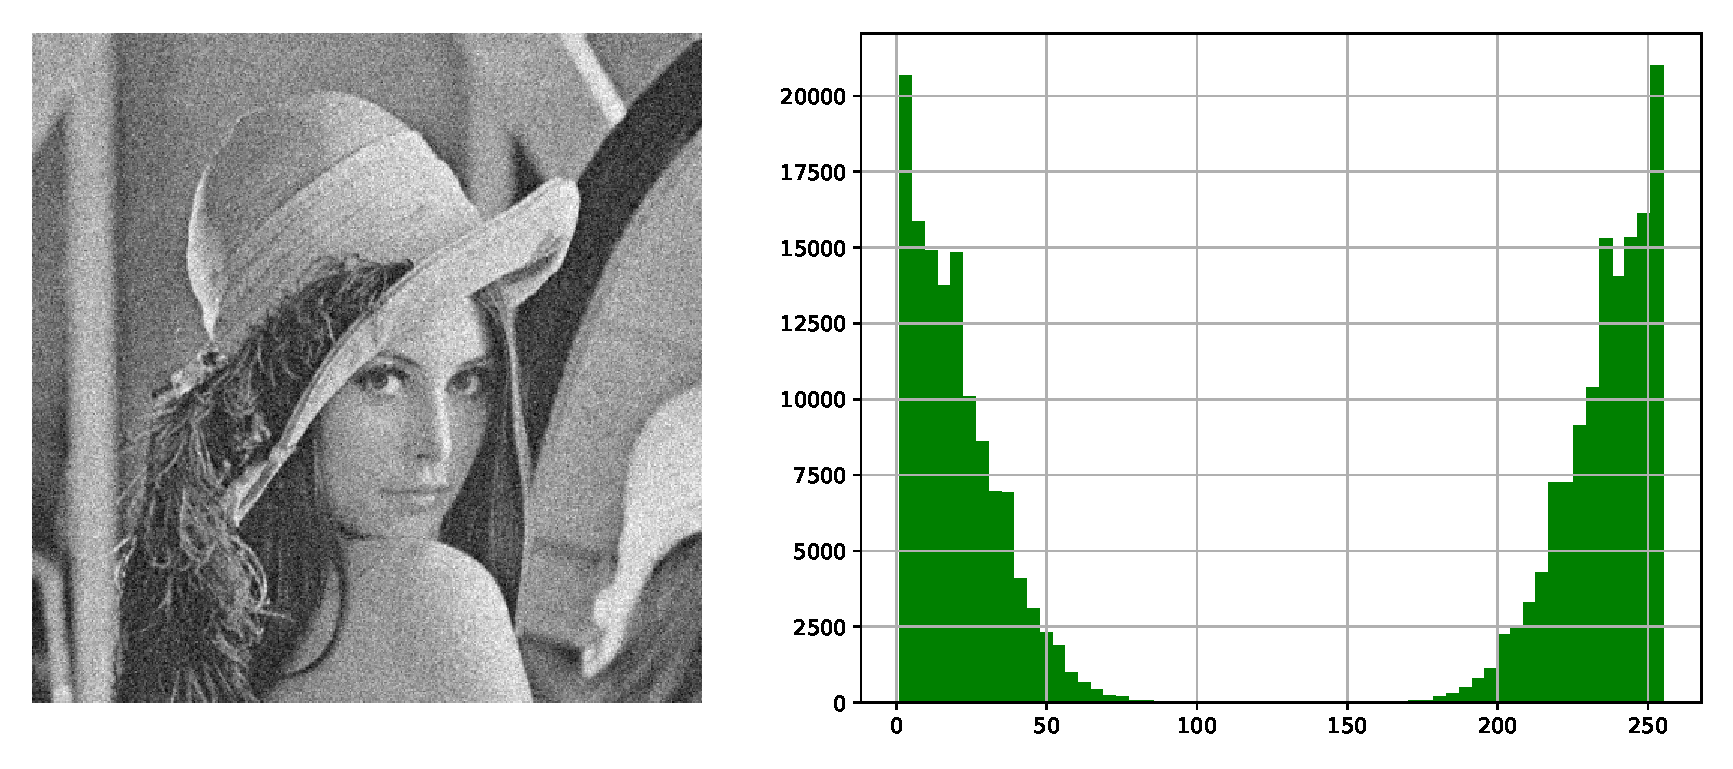
\includegraphics[width=\textwidth]{images/Gaussian_plot.eps}
        \caption{Zgomot Gaussian}
        \label{fig:img4}
    \end{subfigure}
    \hspace{10pt} 
    \begin{subfigure}{0.49\textwidth}
        \centering
        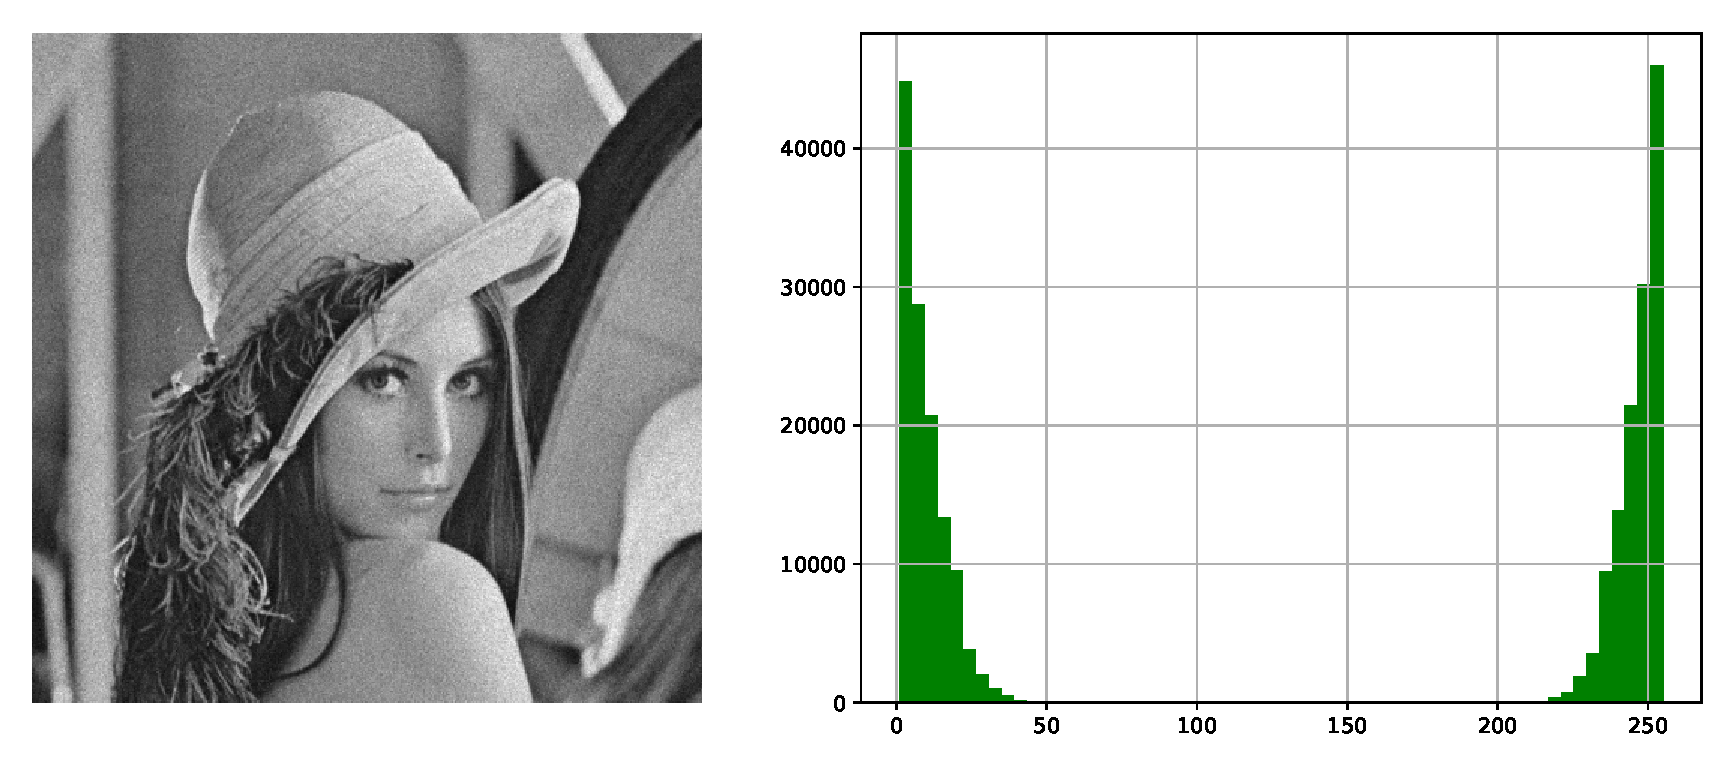
\includegraphics[width=\textwidth]{images/Poisson_plot.eps}
        \caption{Zgomot Poisson}
        \label{fig:img5}
    \end{subfigure}
    \vspace{10pt} 

    \begin{subfigure}{0.49\textwidth}
        \centering
        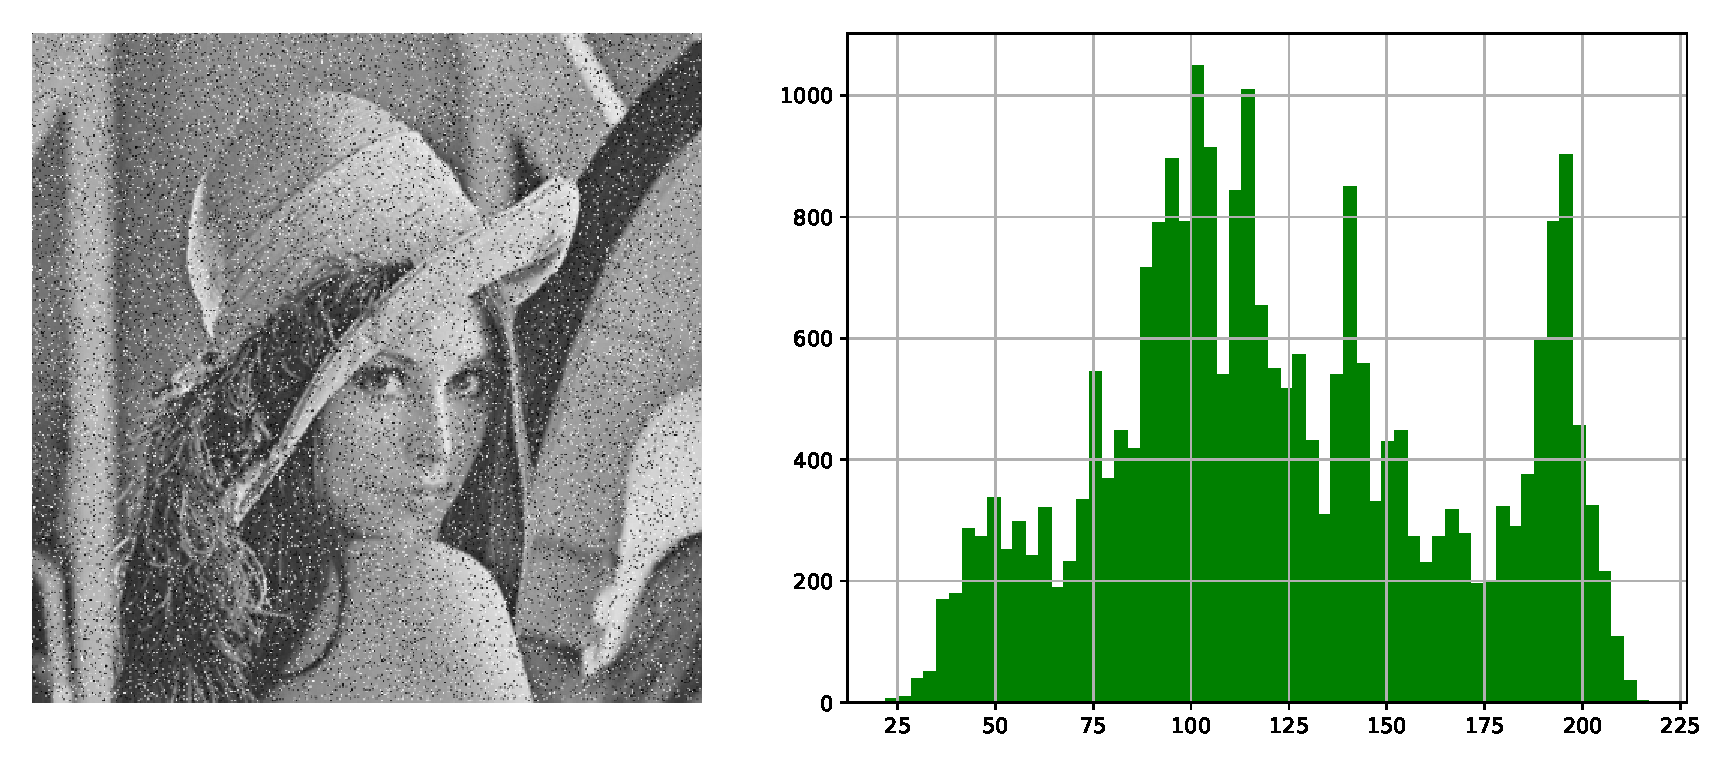
\includegraphics[width=\textwidth]{images/Impulsiv_plot.eps}
        \caption{Zgomot Impulsiv}
        \label{fig:img6}
    \end{subfigure}
	\hspace{10pt} 
    \begin{subfigure}{0.49\textwidth}
        \centering
        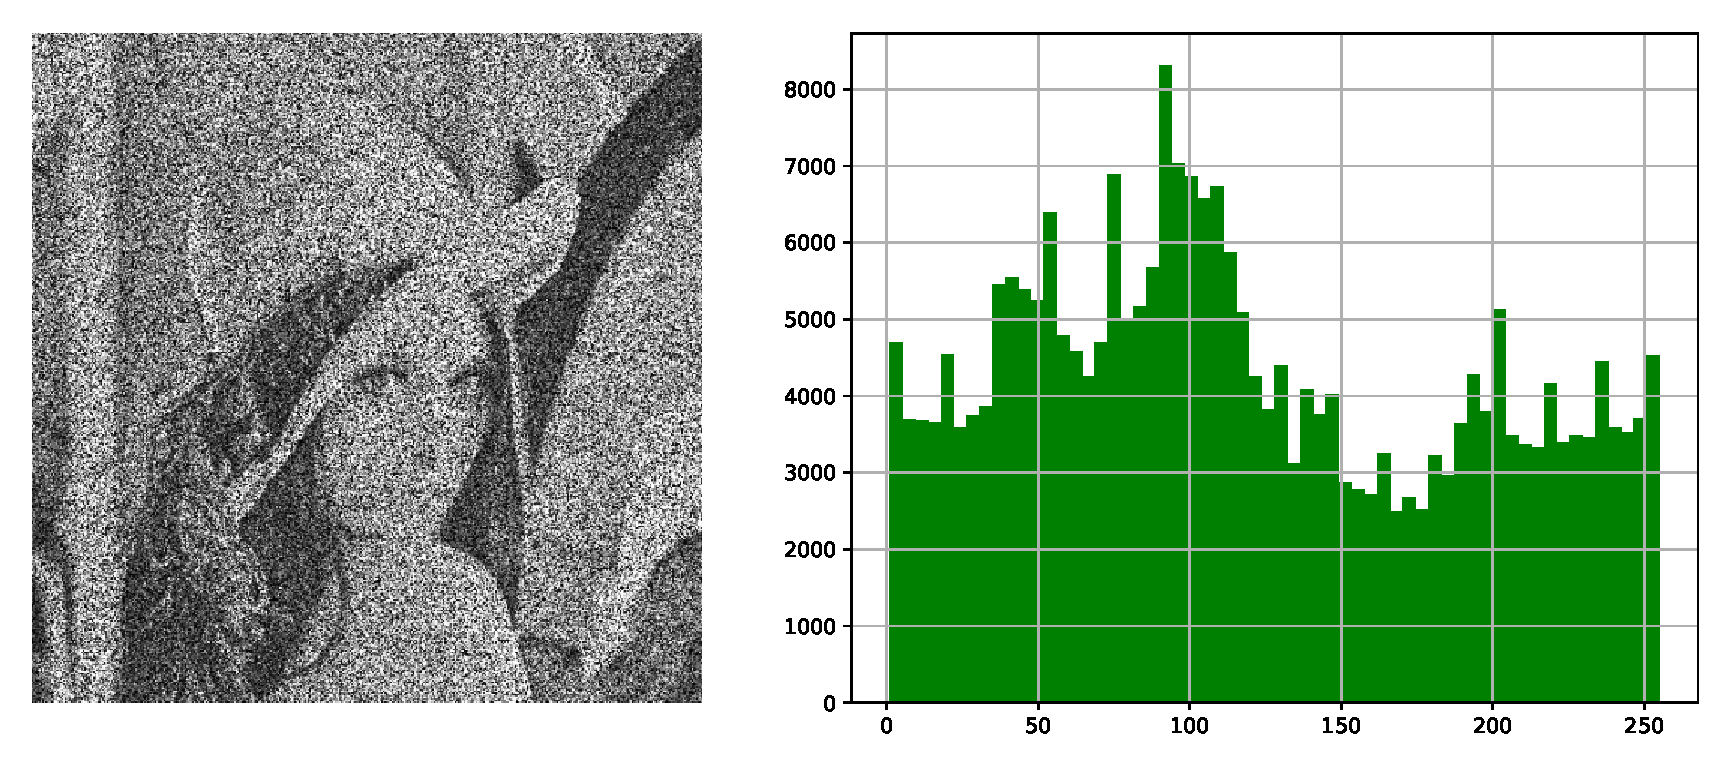
\includegraphics[width=\textwidth]{images/Speckle_plot.eps}
        \caption{Zgomot Speckle}
        \label{fig:img7}
    \end{subfigure}
    \vspace{10pt} 

    \begin{subfigure}{0.49\textwidth}
        \centering
        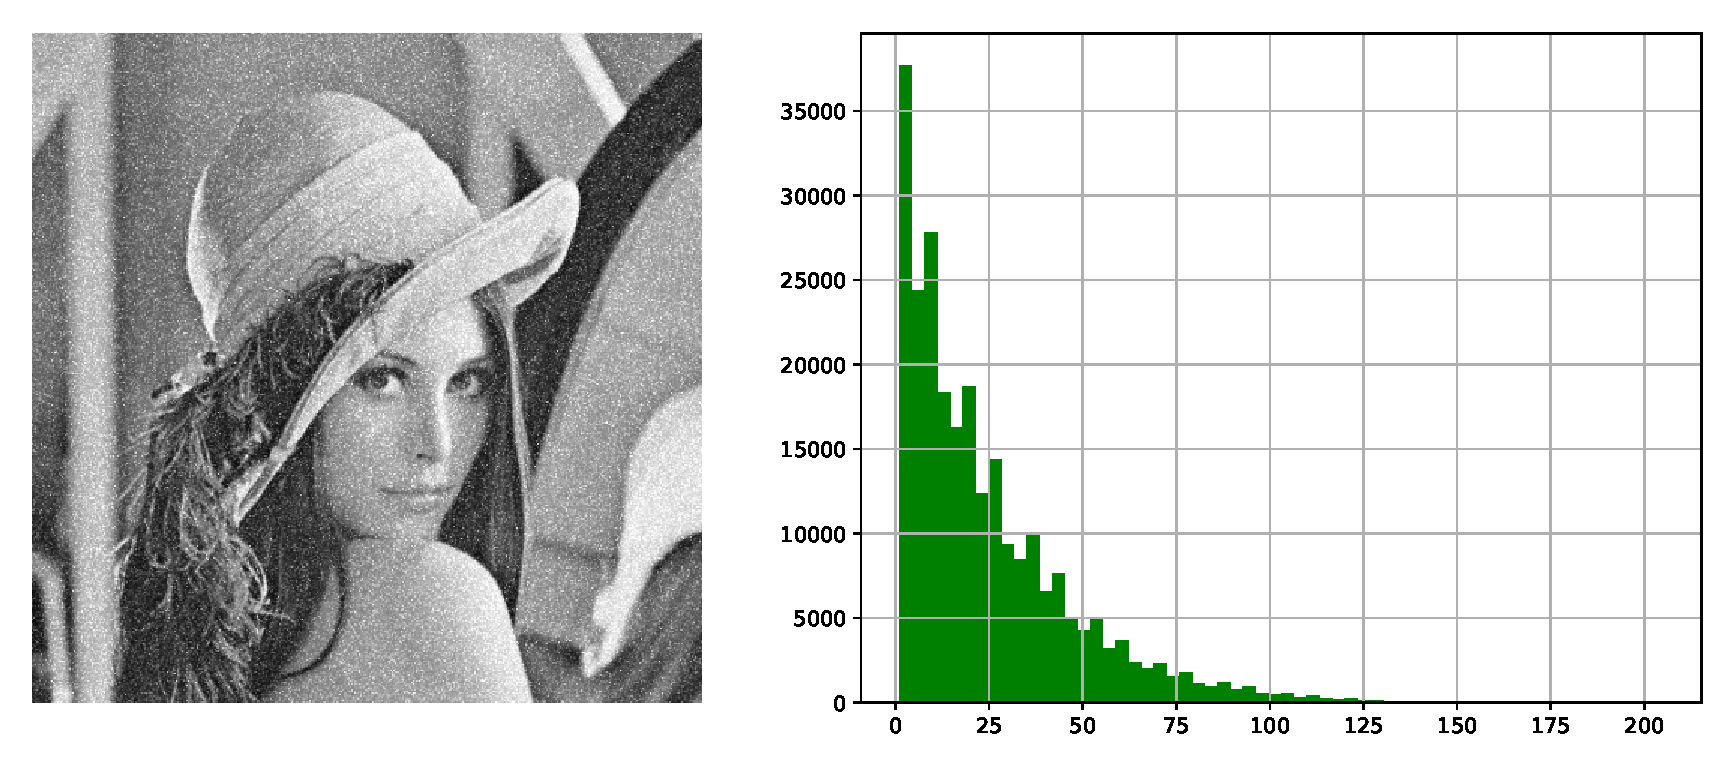
\includegraphics[width=\textwidth]{images/Exponential_plot.eps}
        \caption{Zgomot Exponential}
        \label{fig:img8}
    \end{subfigure}
	\hspace{10pt} 
    \begin{subfigure}{0.49\textwidth}
        \centering
        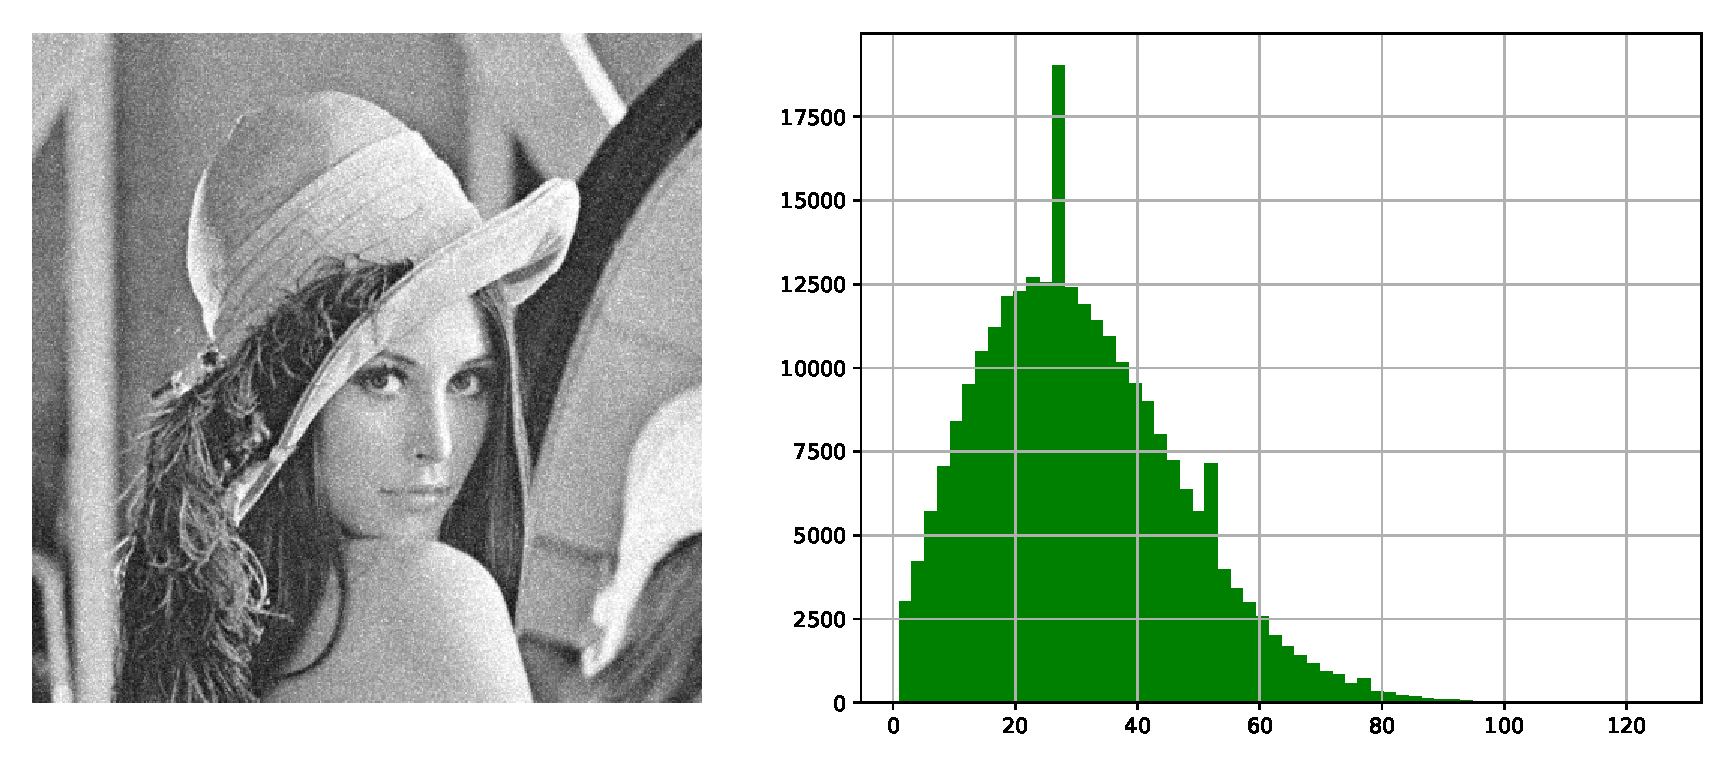
\includegraphics[width=\textwidth]{images/Rayleigh_plot.eps}
        \caption{Zgomot Rayleigh}
        \label{fig:img9}
    \end{subfigure}
    \vspace{10pt} 

    \begin{subfigure}{0.49\textwidth}
        \centering
        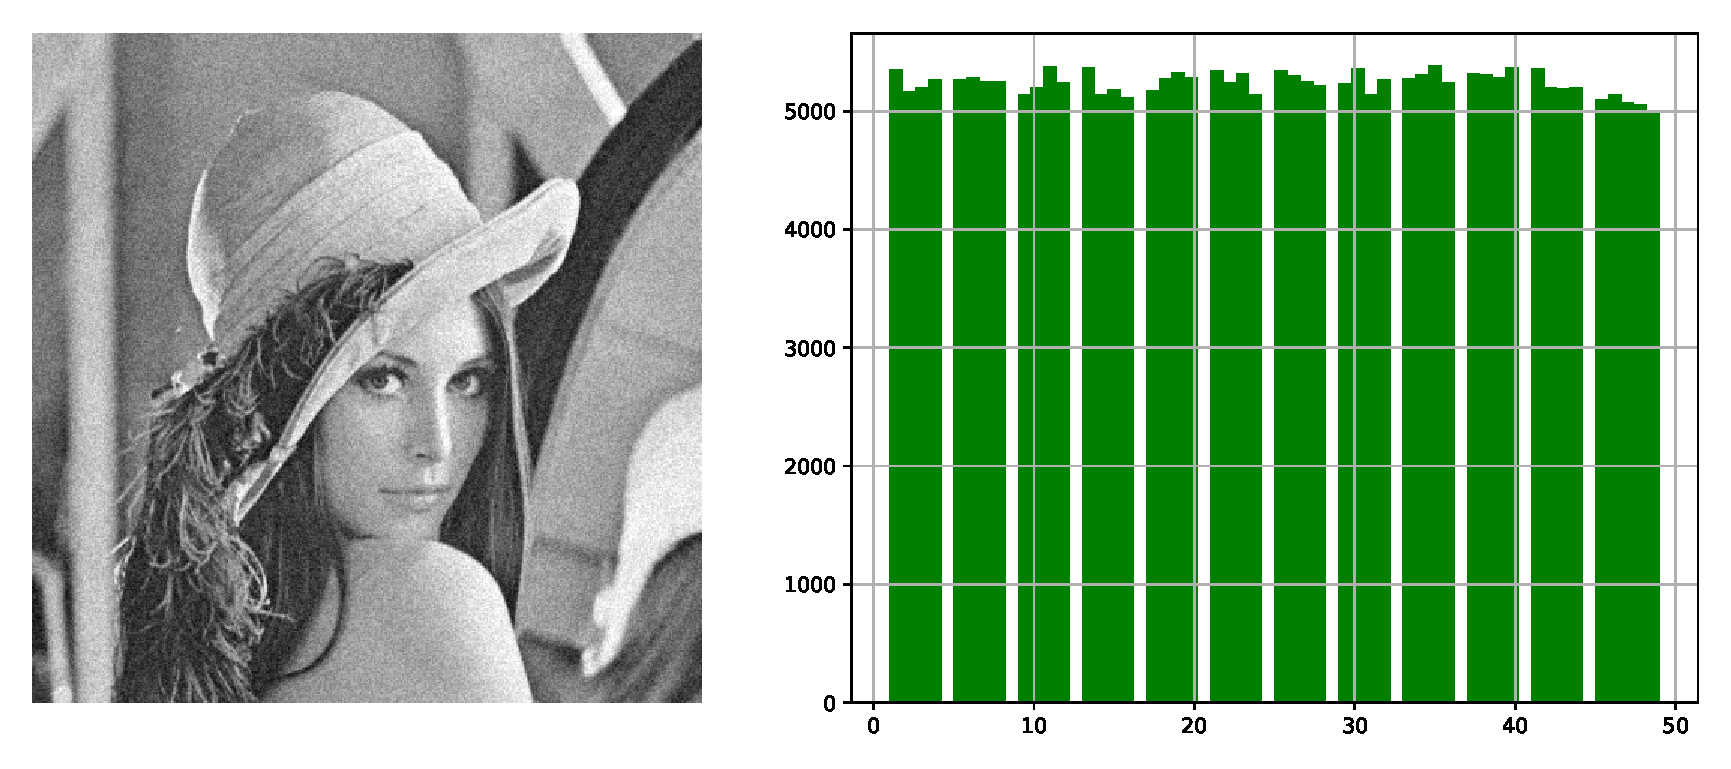
\includegraphics[width=\textwidth]{images/Uniform_plot.eps}
        \caption{Zgomot Uniform}
        \label{fig:img10}
    \end{subfigure}
	\hspace{10pt} 
    \begin{subfigure}{0.49\textwidth}
        \centering
        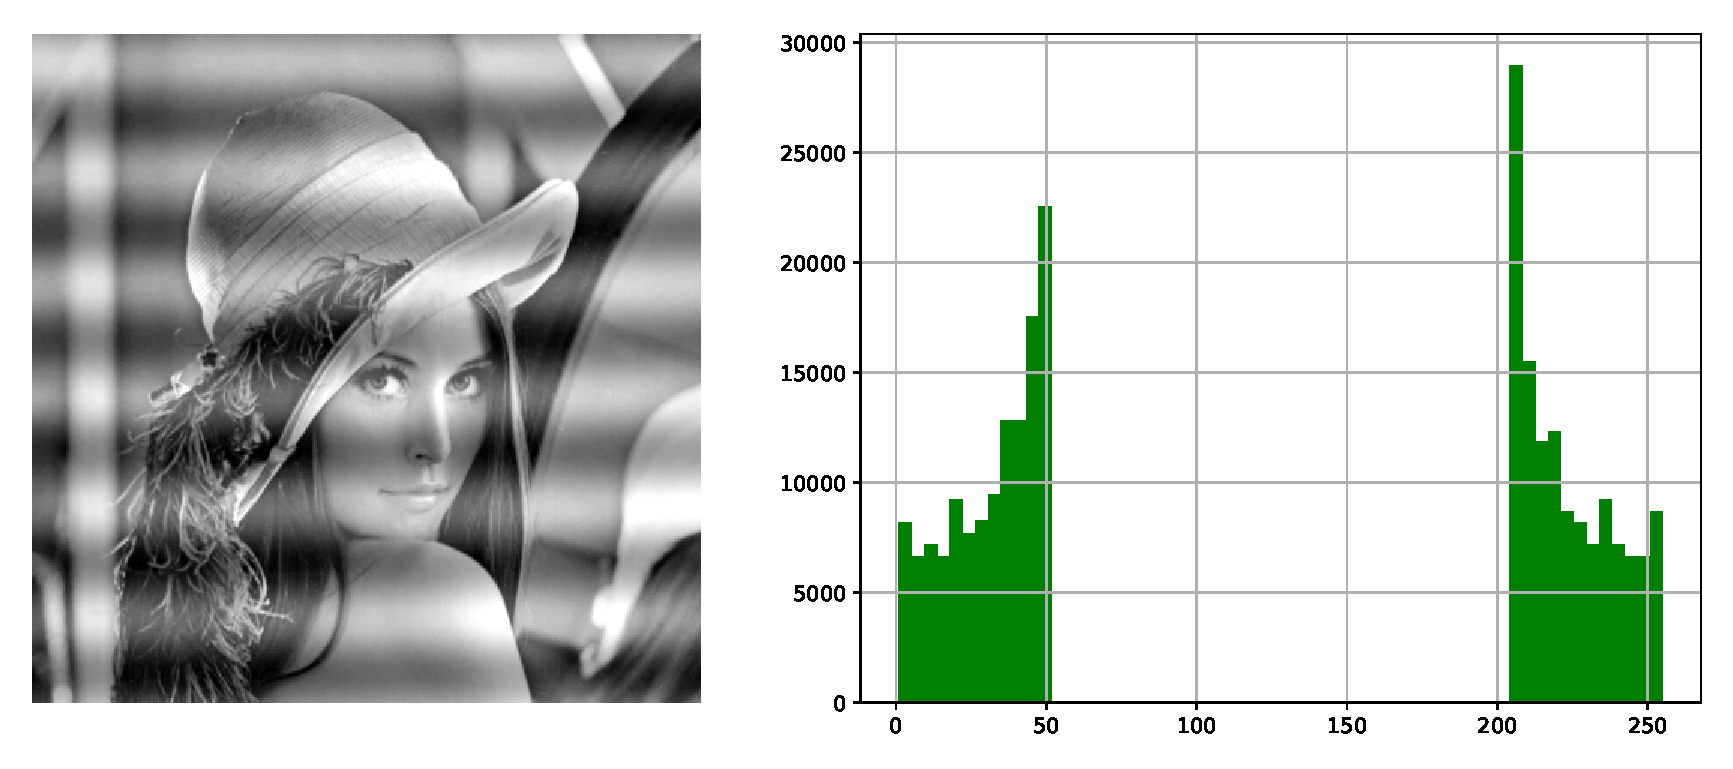
\includegraphics[width=\textwidth]{images/Periodic_plot.eps}
        \caption{Zgomot Periodic}
        \label{fig:img11}
    \end{subfigure}
\end{figure}

\newpage




%%%%%%%%%%%%%%% Algoritmi de reducere a zgomotului din imagini
\section{Algoritmi de reducere a zgomotului din imagini}
\label{sec:algoritmi}

În prezent, se disting două categorii de algoritmi pentru reducerea zgomotului în imagini: Filtrarea Spațială și Filtrarea prin Transformarea Domeniului.\\


\subsection{Filtrarea Spațială}
Filtrarea spațială reprezintă o opțiune eficientă în cazul în care se întâlnește exclusiv zgomot aditiv. Aceasta poate fi ulterior împărțită în două categorii distincte: Filtre Liniare și Filtre Non-Liniare.\\


\subsubsection{Filtre Liniare}
\textbf{Filtrul de Medie} \\
\indent Ideea principală a acestui filtru constă pur și simplu în înlocuirea valorii fiecărui pixel dintr-o imagine cu valoarea medie a pixelilor adiacenți. Filtrul funcționează pe baza algoritmului „ferestrei glisante”, unde fereastra este reprezentată de un kernel de dimensiune ${NXN}$ (cu ${N}$ impar). Fereastra se deplasează pixel cu pixel pe întreaga imagine, calculând media pentru regiunea respectivă. \\
\indent Avantajele acestui filtru sunt implementarea ușoară și eficiența asupra zgomotului gaussian.
Principalul dezavantaj al acestui filtru este faptul că estompează detaliile din imagine și că nu este eficient în tratarea altor tipuri de zgomot, precum zgomotul impulsiv.

\begin{figure}[h!]
    \centering
    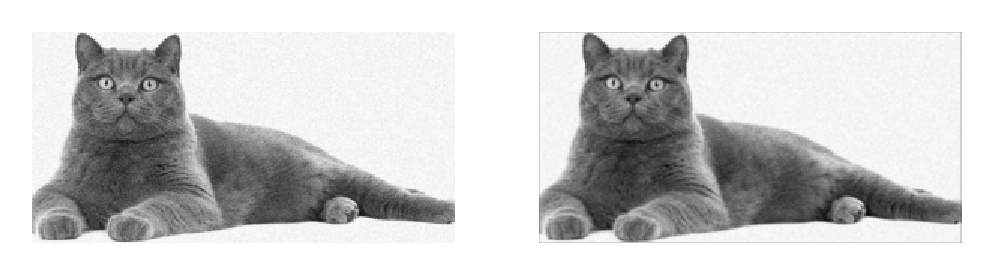
\includegraphics[width=1\textwidth]{images/filtru_medie.eps}
    \caption{Imaginea originală vs Imaginea filtrată}
    \label{fig:img2}
\end{figure}

Prima imagine din Figura \ref{fig:img2} a fost realizată prin adăugarea de zgomot Gaussian (${\sigma=25}$), iar a doua imagine a fost obținută prin aplicarea Filtrului de Medie, cu o dimensiunea a kernelului ${k=5}$. \\[15pt]




\textbf{Filtrul Wiener} \\

\indent Filtrul Wiener este un filtru ce adoptă o abordare statistică pentru a elimina zgomotul dintr-un semnal corupt. Ceea ce îl deosebește este abordarea sa statistică și capacitatea de a obține un răspuns dorit al frecvenței. În loc să se concentreze doar pe reducerea zgomotului, Filtrul Wiener ia în considerare proprietăți spectrale ale semnalului original și ale zgomotului. \\
\indent Pentru a efectua operația de filtrare, este esențial să se cunoască proprietățile spectrale ale semnalului original și ale zgomotului asociat. Filtrul Wiener își propune să obțină un filtru LTI (Linear Time-Invariant) care să furnizeze o ieșire cât mai apropriată de semnalul original.\\
\indent Obiectivul filtrului Wiener este să minimizeze MSE, adică să reducă discrepanța pătratică medie dintre semnalul filtrat și semnalul original. Astfel, proiectarea algoritmului constă în alegerea parametrilor care minimizează MSE pentru a obține o reconstrucție cât mai precisă a semnalului. \\
\indent În acest algoritm, un pixel y din imaginea filtrată este derivat dintr-un pixel x din imaginea de intrare cu zgomot prin următoarea transformare:

\begin{equation}
y = \mu_x + (x - \mu_x) \frac{v_x}{v_x + v_n},
\end{equation} \\
unde ${\mu_x}$ și ${v_x}$ reprezintă media și varianța lui x într-o vecinătate din jurul pixelului, iar ${n_n}$ este varianța zgomotului aditiv, estimată din imaginea de intrare. 
Fiecare pixel de ieșire este suma mediei locale dintr-o vecinătate a pixelului de intrare și a unui termen local de contrast (${x - \mu_x}$) care este scalat astfel încât în regiunile cu detalii ridicate, unde varianța zgomotului (${v_n}$) este mult mai mică decât varianța imaginii (${v_x}$), factorul de scalare este foarte aproape de 1 și pixelul de ieșire ${y}$ este foarte aproape de pixelul de intrare ${x}$ cu puțin filtru, dar în regiunile cu detalii scăzute, unde varianța imaginii este mai mică, pixelul de ieșire tinde să semene mai mult cu media locală (adică este filtrat trece-jos). \\
\indent Vom discuta despre acest filtru mai târziu în această lucrare , unde vom aborda o implementare diferită față de cea spațială.


\subsubsection{Filtre Non-Liniare}
\textbf{Filtrul Median}\\
\indent Se bazează pe aceeași idee ca și filtrul de medie, cu excepția faptului că în loc să se utilizeze media aritmetică, se aplică funcția mediană care înlocuiește fiecare pixel cu valoarea mediană din fereastra respectivă.\\
\indent Filtrul median se dovedește a fi mai robust în fața valorilor extreme comparativ cu filtrul de medie, astfel că este capabil să elimine aceste valori aberante fără a diminua claritatea imaginii.

\begin{figure}[h!]
    \centering
    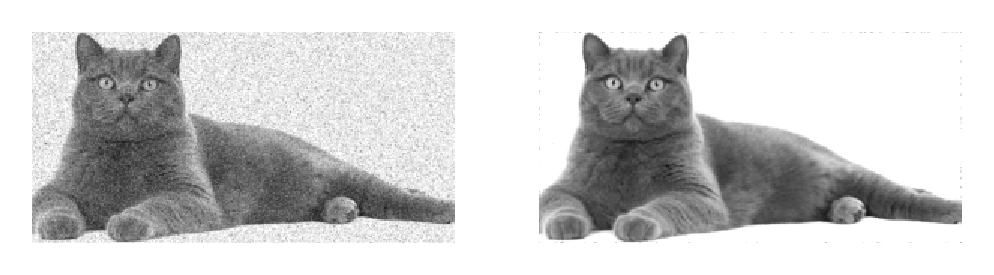
\includegraphics[width=1\textwidth]{images/filtru_median.eps}
    \caption{Imaginea originală vs Imaginea filtrată}
    \label{fig:img3}
\end{figure}

Prima imagine din Figura \ref{fig:img3} a fost realizată prin adăugarea de zgomot Impulsiv, iar a doua imagine a fost obținută prin aplicarea Filtrului Median, cu o dimensiunea a kernelului ${k=5}$. \\[15pt]


\subsubsection{Comparație între Filtrul de Medie și Filtrul Median asupra diferitelor tipuri de zgomote}
\indent În această secțiune, realizăm o comparație între Filtrul de Medie și Filtrul Median aplicate diferitelor tipuri de zgomote. Pentru evaluarea performanței, am utilizat raportul PSNR (Peak Signal-to-Noise Ratio). PSNR cuantifică calitatea unei imagini în comparație cu imaginea originală și este calculat pe baza raportului dintre maximul valorii pătratice a semnalului și eroarea medie pătratică. \\
\indent Fiecare rând al comparației de mai jos conține trei coloane:

\begin{enumerate}
    \item \textbf{Imaginea cu Zgomot:} Prima coloană prezintă imaginea originală cu aplicarea tipului specific de zgomot.

    \item \textbf{Imaginea Obținută prin aplicarea Filtrului de Medie:} A doua coloană conține imaginea rezultată după aplicarea Filtrului de Medie asupra imaginii cu zgomot.

    \item \textbf{Imaginea Obținută prin aplicarea Filtrului Median:} A treia coloană prezintă imaginea rezultată după aplicarea Filtrului Median asupra imaginii cu zgomot.
\end{enumerate}

\begin{figure}[h!]
    \centering
    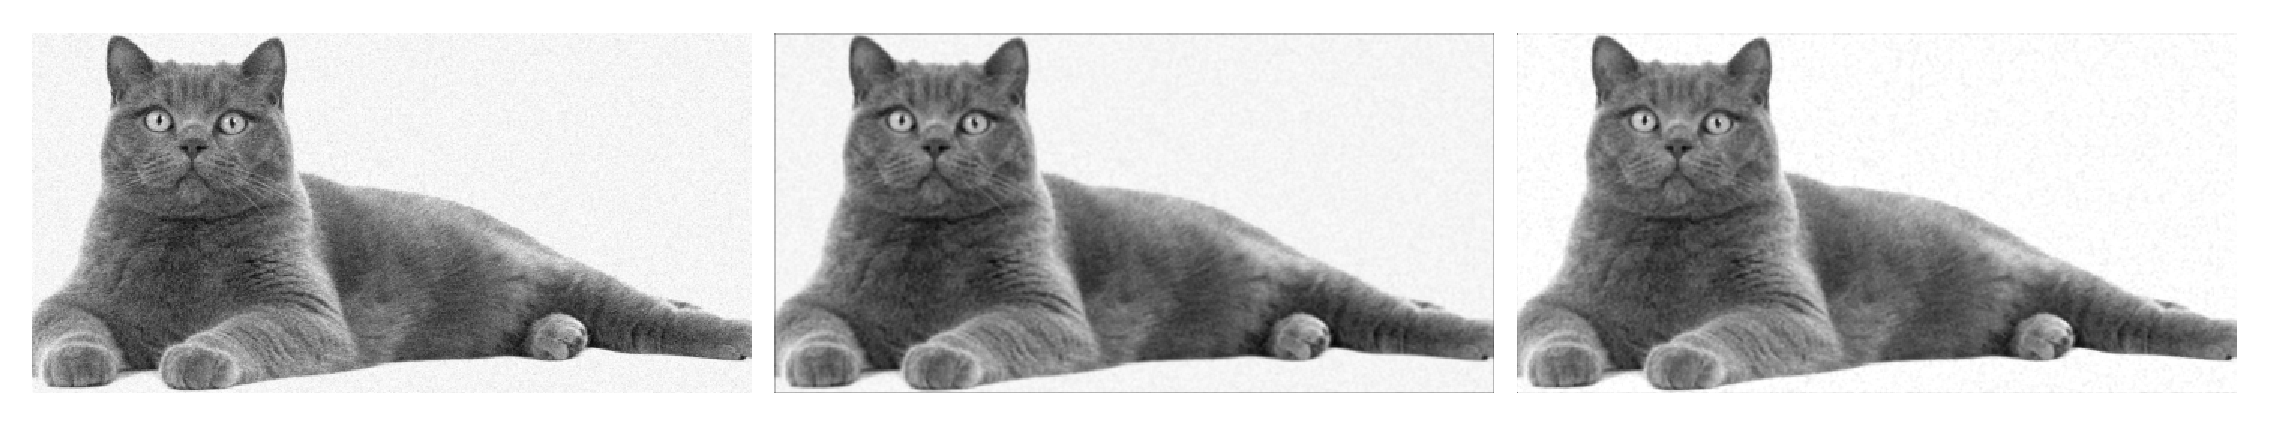
\includegraphics[width=1\textwidth]{images/row_1_filters.eps}
    \caption{Zgomot Gaussian}
    \label{fig:med_gaussian}
\end{figure}
\vspace{10pt} 
\begin{figure}[h!]
    \centering
    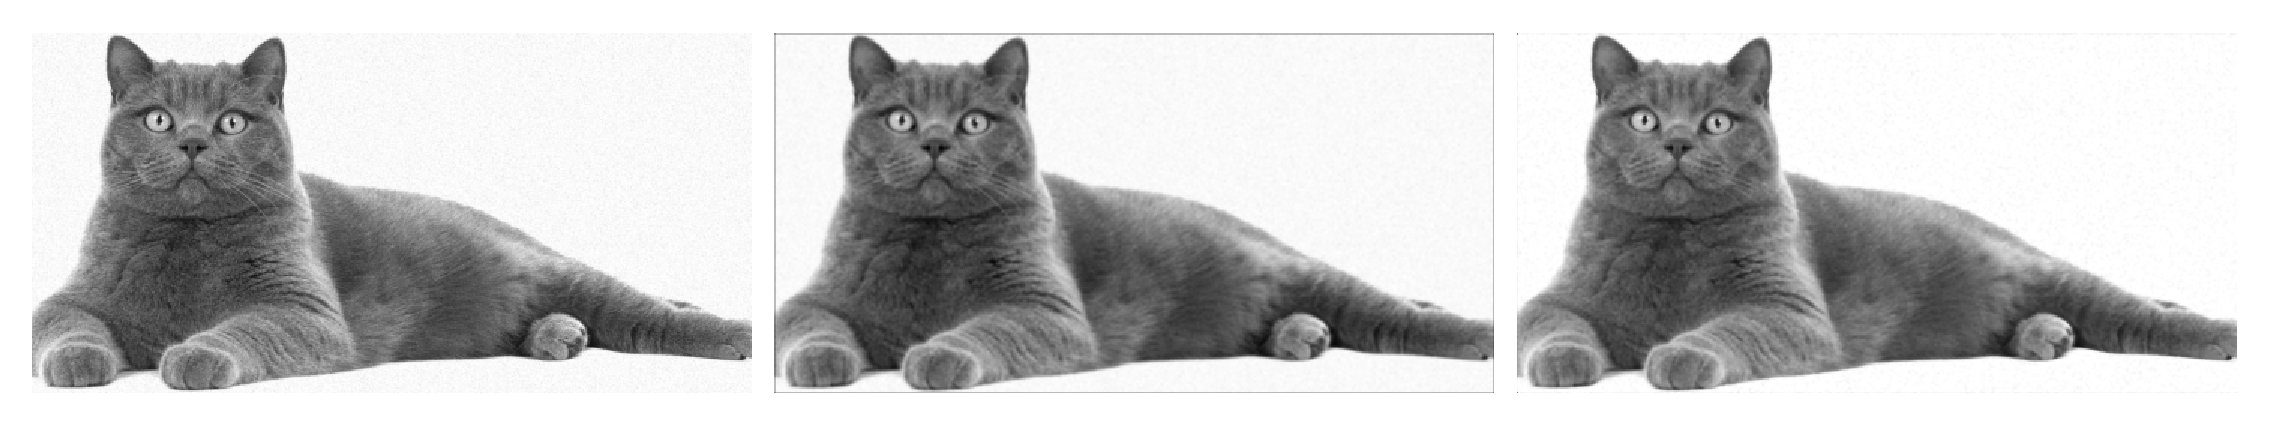
\includegraphics[width=1\textwidth]{images/row_2_filters.eps}
    \caption{Zgomot Poisson}
    \label{fig:med_poisson}
\end{figure}
\vspace{10pt}
\begin{figure}[h!]
    \centering
    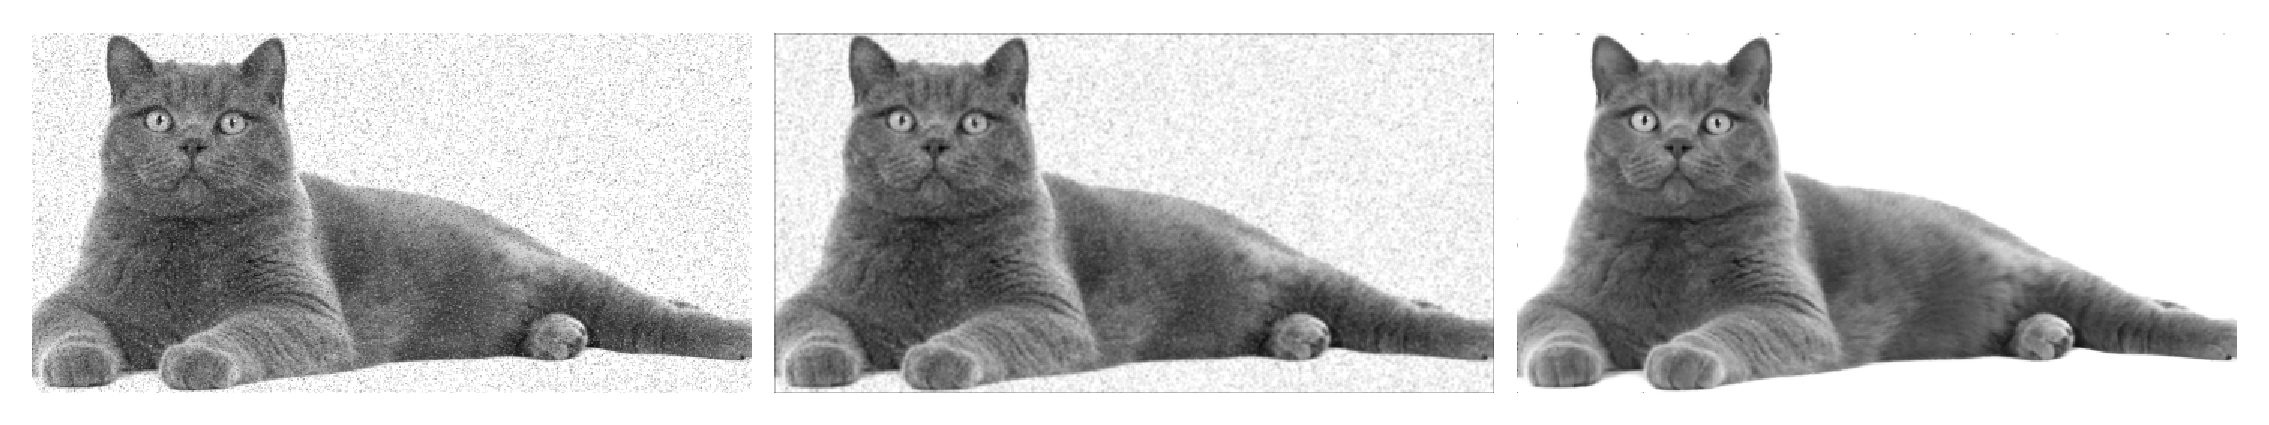
\includegraphics[width=1\textwidth]{images/row_3_filters.eps}
    \caption{Zgomot Impulsiv}
    \label{fig:med_impulsiv}
\end{figure}
\vspace{10pt} \newpage
\begin{figure}[h!]
    \centering
    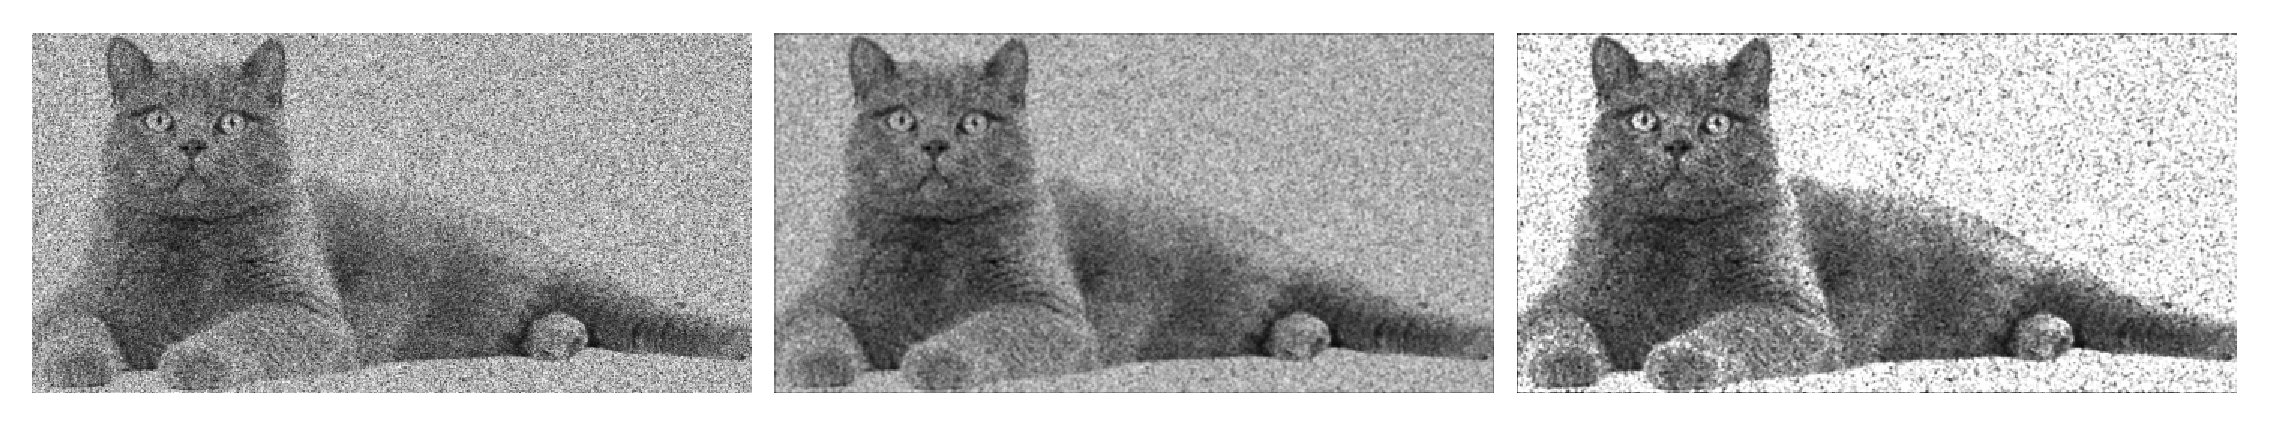
\includegraphics[width=1\textwidth]{images/row_4_filters.eps}
    \caption{Zgomot Speckle}
    \label{fig:med_speckle}
\end{figure}
\vspace{10pt}
\begin{figure}[h!]
    \centering
    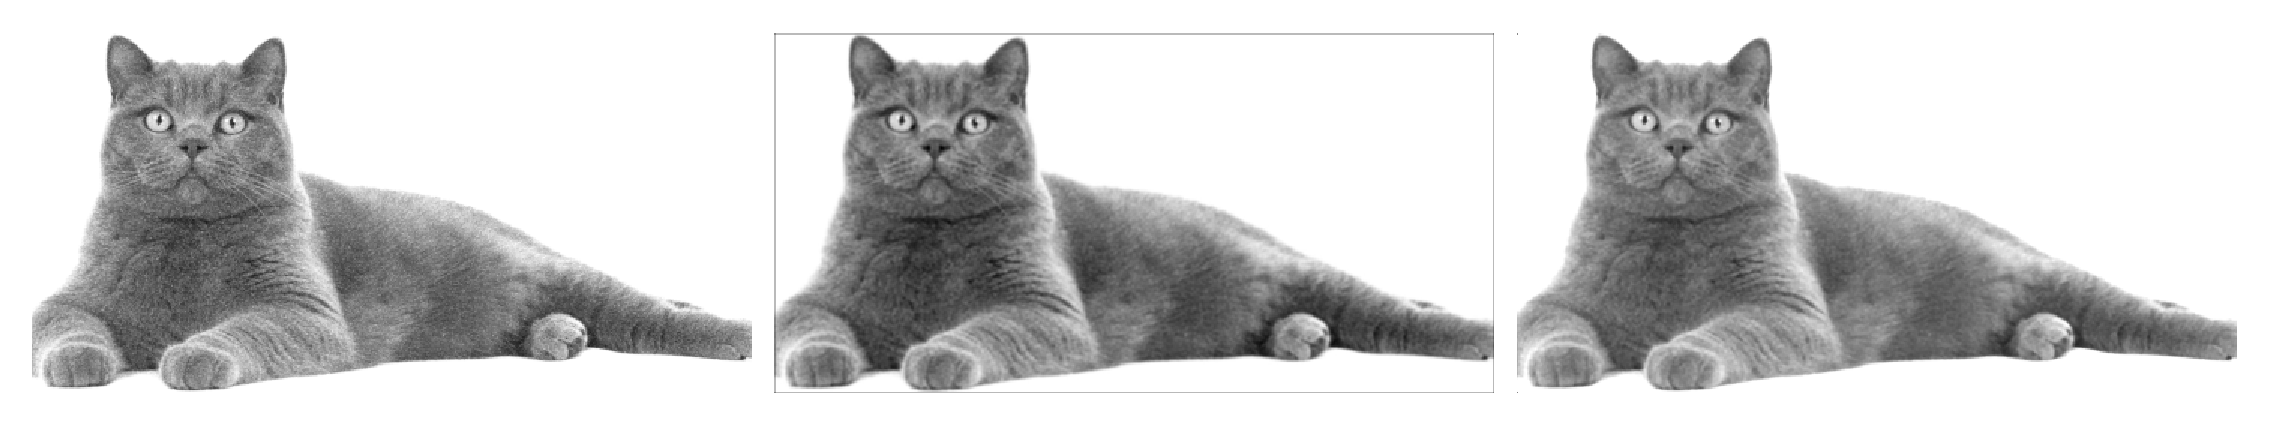
\includegraphics[width=1\textwidth]{images/row_5_filters.eps}
    \caption{Zgomot Exponential}
    \label{fig:med_exponential}
\end{figure}
\vspace{10pt}
\begin{figure}[h!]
    \centering
    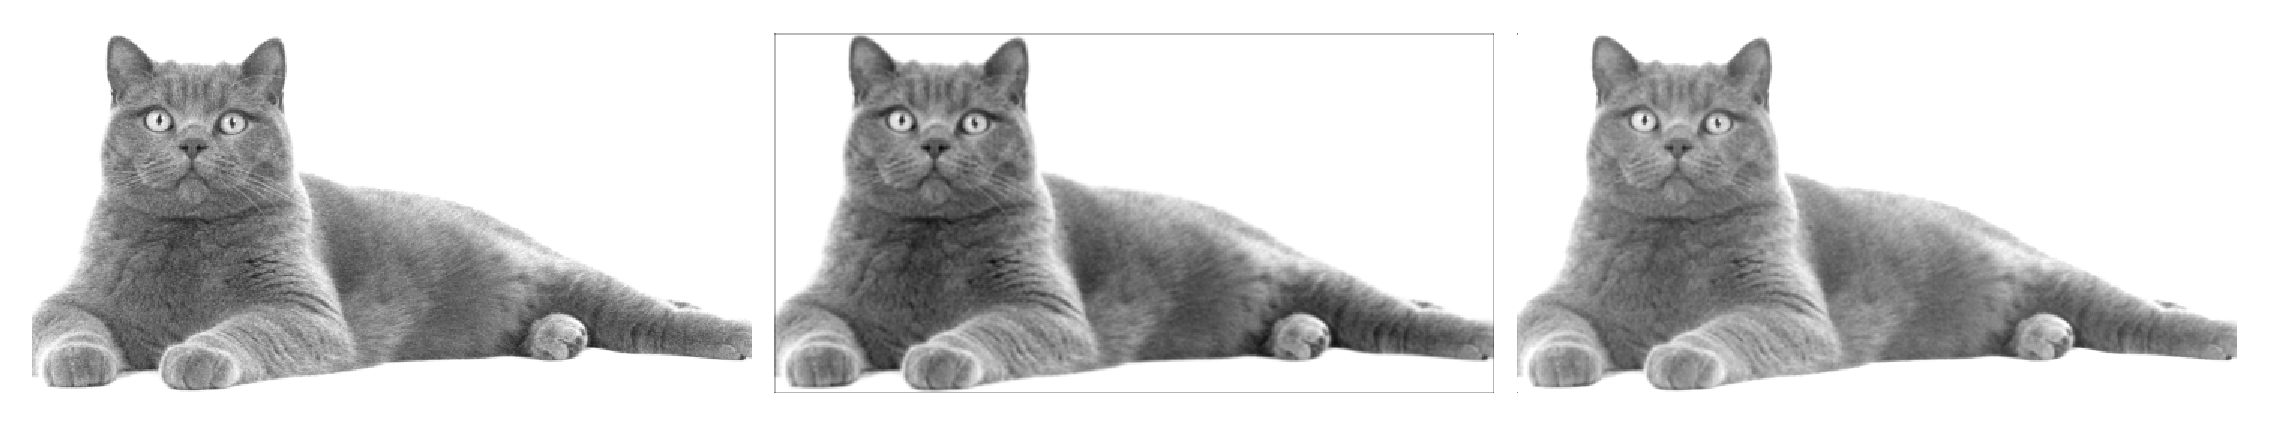
\includegraphics[width=1\textwidth]{images/row_6_filters.eps}
    \caption{Zgomot Rayleigh}
    \label{fig:med_rayleigh}
\end{figure}
\vspace{10pt}
\begin{figure}[h!]
    \centering
    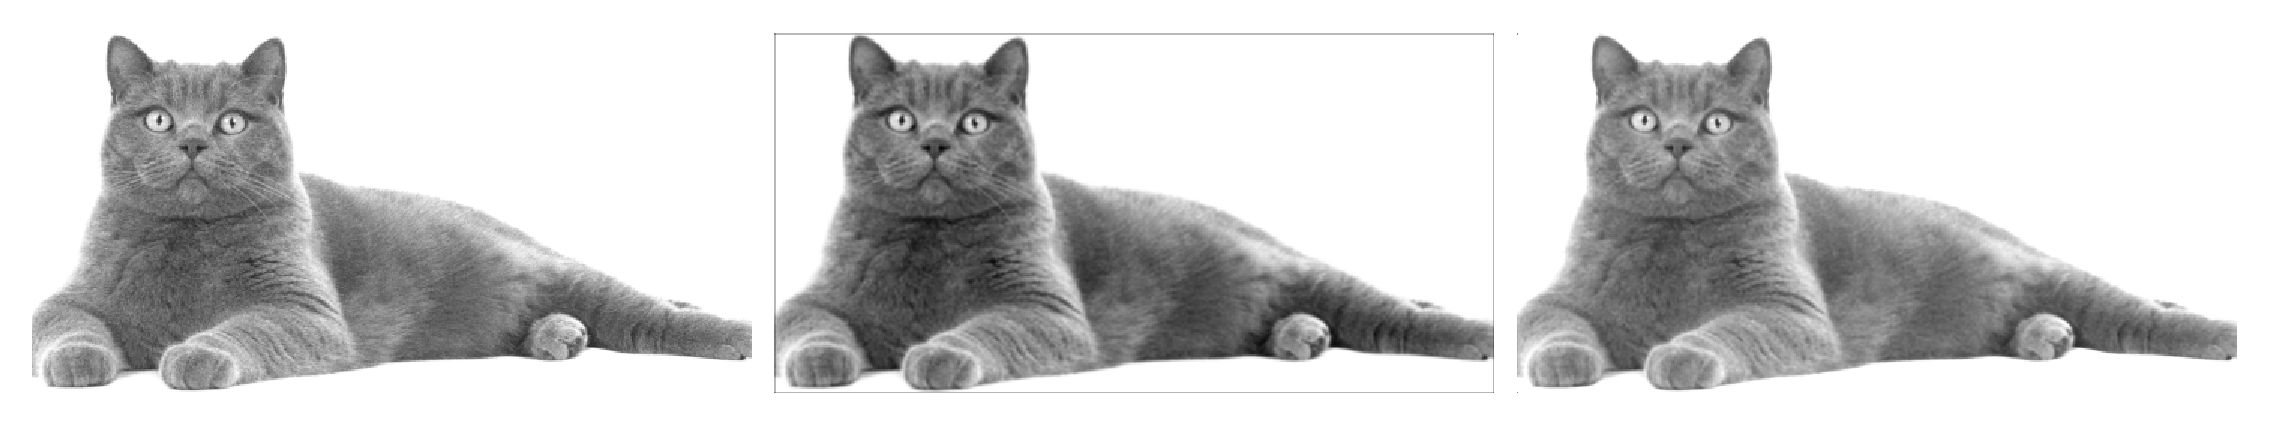
\includegraphics[width=1\textwidth]{images/row_7_filters.eps}
    \caption{Zgomot Uniform}
    \label{fig:med_uniform}
\end{figure}
\vspace{10pt} \newpage

\begin{figure}[h!]
    \centering
    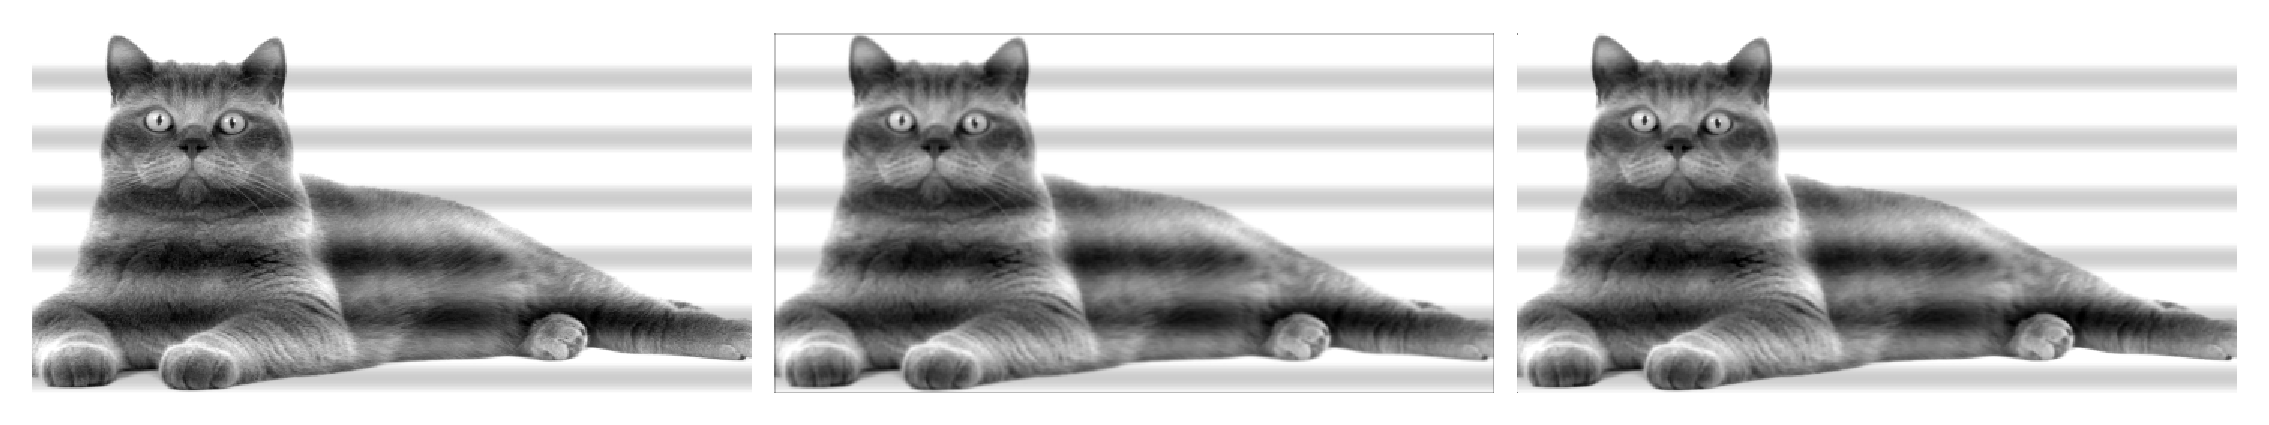
\includegraphics[width=1\textwidth]{images/row_8_filters.eps}
    \caption{Zgomot Periodic}
    \label{fig:med_periodic}
\end{figure}
\vspace{15pt}

\begin{table}[h!]
    \centering
    \begin{tabular}{|c|c|c|c|}
        \hline
        \thead{\textbf{Tip de zgomot}} & \thead{\textbf{PSNR imaginea} \\ \textbf{cu zgomot}} & \thead{\textbf{PSNR imaginea} \\ \textbf{cu Filtru de Medie}} & \thead{\textbf{PSNR imaginea} \\ \textbf{cu Filtru Median}} \\
        \hline
        Gaussian & 21.44 & 23.76 & 26.16 \\
        \hline
        Poisson & 27.36 & 24.66 & 26.98 \\
        \hline
        Impulsiv & 14.23 & 22.25 & 27.02 \\
        \hline
        Speckle & 7.35 & 12.09 & 15.49 \\
        \hline
        Exponential & 20.65 & 21.38 & 22.87 \\
        \hline
        Rayleigh & 20.44 & 20.07 & 20.61 \\
        \hline
        Uniform & 22.19 & 21.38 & 21.89 \\
        \hline
        Periodic & 18.41 & 17.60 & 17.90 \\
        \hline
    \end{tabular}
    \caption{Valorile PSNR pentru diferite tipuri de zgomote și Filtru de Medie și Median}
    \label{tab:psnr_values}
\end{table}



\subsection{Filtrarea prin Transformarea Domeniului}
Filtrarea prin transformarea domeniului reprezintă o tehnică de prelucrare a semnalelor, în care datele sunt transformate din domeniul spațial în alt domeniu matematic (domeniul frecvenței sau al undelor) pentru a eficientiza operațiile de filtrare, cum ar fi convoluția. Această transformare permite utilizarea optimă a tehnicilor de filtrare, iar rezultatul poate fi convertit înapoi in domeniul original, fără să existe informații pierdute. \\

\subsubsection{Filtrarea în Domeniul Frecvenței}
Se referă la utilizarea filtrelor trece-jos folosind Transformata Fourier. Zgomotul este eliminat prin stabilirea unui prag de frecvență și aplicarea acestuia asupra imaginii în domeniul frecvenței, unde componenta zgomotului este decorelată de semnalul util.\\
\indent Principalul dezavantaj al Transformatei Fourier Rapide constă în faptul că informațiile marginale sunt distribuite pe întregul spectru al frecvenței, și nu pot fi localizate în timp sau spațiu. Prin urmare, filtrul trece-jos afectează imaginea prin estomparea marginilor (muchiilor). Aici apare conceptul de localizare a semnalului în timp și frecvență folosind Transformata Wavelet, ce oferă o metodă deosebit de utilă pentru reducerea zgomotului în imagini atunci când păstrarea muchiilor este importantă. \\

\indent Am aplicat procesul de filtrare în domeniul frecvenței pentru a elimina zgomotul din imaginea cu pisica british fold folosită și în capitolele anterioare. În prima etapă a acestui proces am adăugat zgomot Gaussian imaginii originale, după care am aplicat Transformata Fourier 2D asupra imaginii cu zgomot, transpunând astfel imaginea din domeniul spațial în cel al frecvenței. \\
\indent La pasul al doilea am proiectat un Filtru Trece-Jos și l-am aplicat asupra imaginii zgomotoase, având ca scop eliminarea componentelor de frecvență înaltă, ce corespund zgomotului din imagine.

\begin{figure}[h!]
    \centering
    \includegraphics[width=1\textwidth]{images/low_pass_filter.eps}
    \caption{Filtru trece-jos}
    \label{fig:low_pass_filter}
\end{figure}

\begin{figure}[h!]
    \centering
    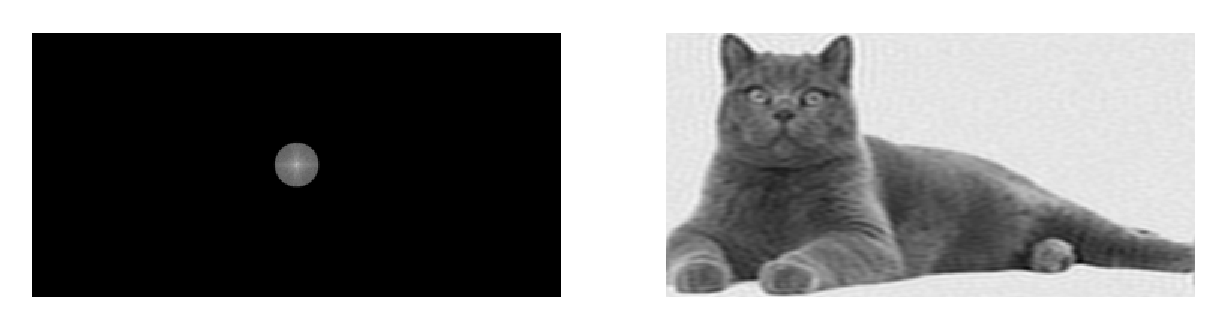
\includegraphics[width=1\textwidth]{images/inverse_fourier_transform.eps}
    \caption{Transformata Fourier inversă}
    \label{fig:inverse_fourier_transform}
\end{figure} \newpage

\indent În ultima etapă a acestui proces am aplicat Transformata Fourier Inversă pentru a obține imaginea fără zgomot, revenindu-se astfel din domeniul frecvenței în cel spațial.

\begin{figure}[h!]
    \begin{subfigure}{0.49\textwidth}
        \centering
        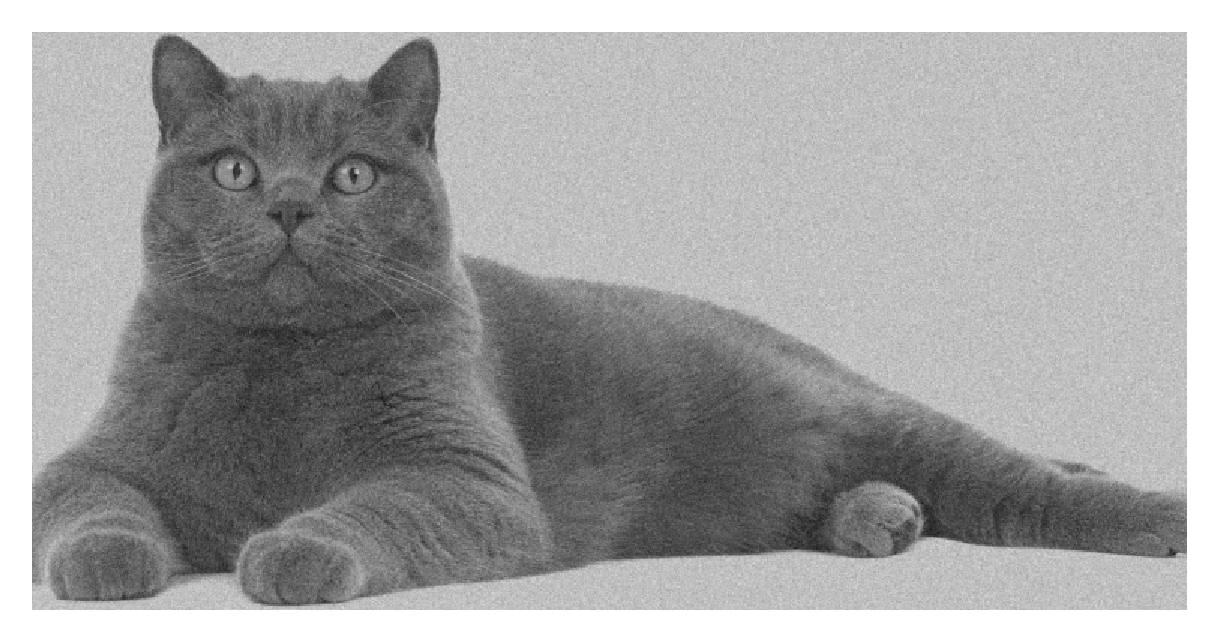
\includegraphics[width=1\textwidth]{images/noisy_image.eps}
        \caption{Imaginea cu zgomot}
        \label{fig:noisy_image}
    \end{subfigure}
    \hspace{10pt}
    \begin{subfigure}{0.49\textwidth}
        \centering
        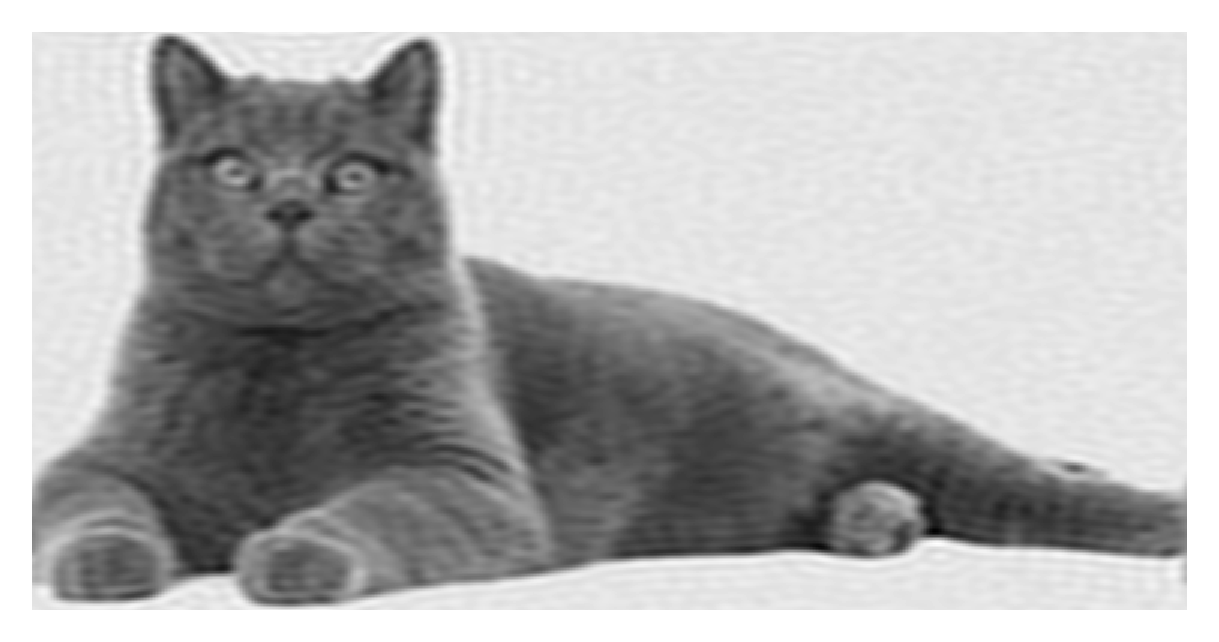
\includegraphics[width=1\textwidth]{images/denoised_dft.eps}
        \caption{Imaginea filtrată}
        \label{fig:denoised_dft}
    \end{subfigure}
    \vspace{5pt}
\end{figure}

\subsubsection{Filtrarea în Domeniul Wavelet}
Operarea în domeniul Wavelet este preferată deoarece Transformata Wavelet Discretă concentrează energia semnalului într-un număr mic de coeficienți, prin urmare, utilizarea DWT asupra imaginii zgomotoase rezultă un număr mic de coeficienți ce au un raport semnal/zgomot (SNR) ridicat, în timp ce un număr relativ mare de coeficienți au un SNR scăzut. După eliminarea coeficienților cu SNR scăzut, imaginea este reconstruită cu ajutorul IDWT (Inversa Transformării Wavelet Discrete), ce rezultă eliminarea sau filtrarea zgomotului. Metodele Wavelet au un avantaj semnificativ, acela de a localiza simultan timpul cu frecvența, fiind astfel o alegere potrivită pentru reducerea zgomotului din imagine.

Aplicăm procesul de eliminare a zgomotului folosind Transformata Wavelet pe imaginea pisica british cu zgomotul Gaussian. În prima etapă, imaginea este descompusă într-o serie de coeficienți wavelet de tip „haar”, care reprezintă detaliile și aproximările la diferite niveluri de scală. Nivelul de descompunere indică de câte ori este aplicată transformata wavelet asupra imaginii. \\
\indent După obținerea coeficienților, stabilim un prag care acționează ca limită pentru coeficienții mici, considerați a fi asociați zgomotului. Cu ajutorul acestui prag, aplicăm o tehnică de umplere numită „soft thresholding” asupra coeficienților. Cu alte cuvinte, coeficienții cu valorile sub prag sunt reduși sau eliminați, având ca impact reducerea zgomotului. \\
\indent În final, imaginea este reconstruită utilizând inversa Transformatei Discrete Wavelet. Acest proces permite păstrarea detaliilor, eliminând în același timp componentele zgomot.


\begin{figure}[h!]
    \centering
    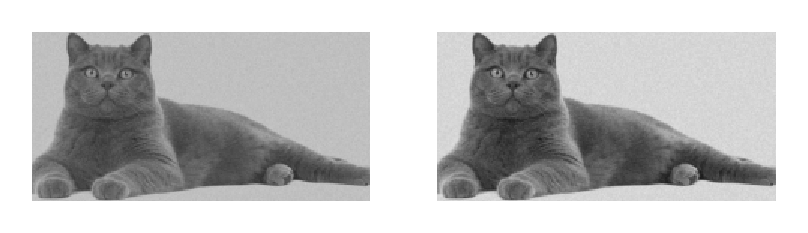
\includegraphics[width=1\textwidth]{images/dwt_img1.eps}
    \caption{Wavelet haar, level=1}
    \label{fig:dwt_img1}
\end{figure}
\begin{figure}[h!]
    \centering
    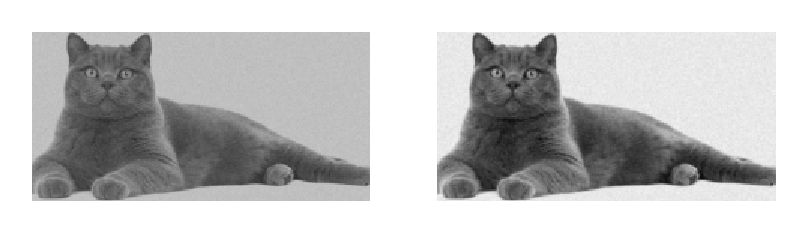
\includegraphics[width=1\textwidth]{images/dwt_img2.eps}
    \caption{Wavelet haar, level=2}
    \label{fig:dwt_img2}
\end{figure}

\begin{figure}[h!]
    \centering
    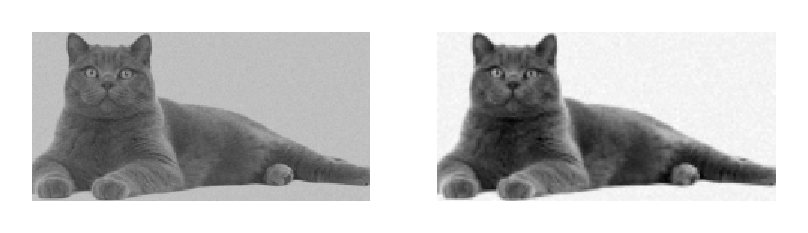
\includegraphics[width=1\textwidth]{images/dwt_img3.eps}
    \caption{Wavelet haar, level=3}
    \label{fig:dwt_img3}
\end{figure}

\newpage
\section{Restituirea imaginilor}
\label{sec:restituirea_imaginilor}

\subsection{Deconvoluția Wiener}
\label{sec:deconv_wiener}

Filtrul Wiener a fost unul dintre primele metode dezvoltate pentru reducerea zgomotului aditiv aleator în imagini. Acesta funcționează pe premisa că zgomotul aditiv este un proces aleatoriu staționar, independent de locația pixelului; algoritmul minimizează eroarea dintre imaginea originală și cea reconstruită. Filtrul Wiener este un filtru trece-jos, dar în loc să aibă o singură frecvență de tăiere, este un filtru variabil în spațiu, proiectat să folosească o tăiere redusă în regiunile cu detalii scăzute și o tăiere mare pentru a păstra detaliile în regiunile cu margini sau alte caracteristici cu variație mare. Dimensiunea ferestrei determină tăierea frecvenței generale: ferestrele mai mari corespund unor frecvențe de tăiere mai scăzute și, prin urmare, mai multă estompare și reducere a zgomotului.\\

Având o imagine x și un kernel de convoluție invariant la deplasare sau o funcție de răspândire a punctelor (PSF) c, se formează o imagine 2D b conform următoarei relații:
\begin{equation}
b = cx + \eta,
\label{eq:wiener_deconv_form_1}
\end{equation}

Aici, măsurătorile sunt afectate de un termen de zgomot aditiv, independent de semnal ${\eta}$.
Teorema de convoluție afirmă că ecuația \ref{eq:wiener_deconv_form_1} poate fi scrisă similar ca o înmulțire în domeniul Fourier:
\begin{equation}
b = \mathcal{F}^{-1}\{\mathcal{F}\{c\} \cdot \mathcal{F}\{x\}\},
\label{eq:wiener_deconv_form_2}
\end{equation}
unde · reprezintă produsul element cu element. Se observă că Ecuțiile \ref{eq:wiener_deconv_form_1} și \ref{eq:wiener_deconv_form_2} sunt echivalente numeric doar atunci când convoluția este efectuată cu condiții de limită circulare.\\
\indent Deconvoluția este problema de a găsi o estimare ${\tilde{x}}$ a imaginii latente b din măsurători neclare, cu zgomot.

Principala problemă a filtrării inverse este că zgomotul de măsurare este ignorat pentru reconstrucție. Filtrul Wiener aplicat problemei de deconvoluție adaugă un factor de amortizare la filtrul invers:
\begin{equation}
\tilde{x} = \mathcal{F}^{-1}\left\{\frac{|\mathcal{F}\{c\}|^2}{|\mathcal{F}\{c\}|^2 + \frac{1}{\text{SNR}}} \cdot \frac{\mathcal{F}\{b\}}{\mathcal{F}\{c\}}\right\},
\label{eq:wiener_deconv_form_3}
\end{equation}
unde SNR reprezintă raportul semnal-zgomot. Dacă nu există zgomot în măsurători, SNR-ul este infinit de mare. În această situație particulară, filtrarea Wiener este echivalentă cu filtrarea inversă. În toate celelalte cazuri, Ecuatia \ref{eq:wiener_deconv_form_3} adaugă un factor de amortizare pe frecvență care necesită cunoașterea magnitudinii semnalului și a densității spectrale de putere a zgomotului pentru fiecare frecvență. O aproximare comună pentru aceasta este de a alege termenul de semnal ca intensitate medie a imaginii și termenul de zgomot ca deviația standard a distribuției de zgomot ${\eta}$.\\

Am selectat imaginea din Figura \ref{fig:wiener_im1} ca imagine de test, iar Figura \ref{fig:wiener_im2} a fost generată prin adăugarea de zgomot. Procesul a implicat adăugarea a 30\% din deviația standard a imaginii originale la fiecare pixel al imaginii convoluționate. Această adiție a fost efectuată înmulțind valorile rezultate cu numere aleatoare generate dintr-o distribuție normală standard. În continuare, Figura \ref{fig:wiener_im3} a fost obținută prin aplicarea filtrului Wiener. Observăm că, deși zgomotul a fost redus semnificativ în imaginea filtrată, raportul PSNR (Peak Signal-to-Noise Ratio) a înregistrat o scădere. Este important de menționat că, în cazul Figurii \ref{fig:img4}, deși filtrul Wiener a îmbunătățit vizibil claritatea imaginii, PSNR a înregistrat o scădere, sugerând că raportul dintre semnal și zgomot nu este atât de favorabil. 

Fiecare imagine din figurile de mai jos are atașat spectrul de frecvență, ce evidențiază intensitatea frecvențelor din imagine. Spectrul de frecvență a fost obținut prin aplicarea unei transformate Fourier bidimensionale. După cum se observă din graficul spectrului de frecvență a imaginii filtrate prezența frecvențelor înalte indica faptul că filtrul Wiener a reușit să atenueze efectele negative ale zgomotului, menținând totuși detaliile din imaginea inițialăgraficul spectrului.

\begin{figure}[h!]
    \centering
    \includegraphics[width=0.75\textwidth]{images/wiener_im1.eps}
    \caption{Imaginea originală}
    \label{fig:wiener_im1}
\end{figure}
\newpage

\begin{figure}[h!]
    \centering
    \includegraphics[width=0.75\textwidth]{images/wiener_im2.eps}
    \caption{Imaginea cu zgomot}
    \label{fig:wiener_im2}
\end{figure}

\begin{figure}[h!]
    \centering
    \includegraphics[width=0.75\textwidth]{images/wiener_im3.eps}
    \caption{Imaginea filtrată}
    \label{fig:wiener_im3}
\end{figure}


%%%%%%%%%%%%%%% Filtrul CLS
\subsection{Filtrul CLS}
\label{sec:cls}
\indent Filtrul CLS (Constrained Least Squares) încearcă să obțină un compromis între accentuarea imaginii și îmbunătățirea zgomotului aleator prin maximizarea netezimii imaginii restaurate, respectând în același timp o constrângere la cât de bine (în sensul diferențelor medii pătratice) imaginea restaurată se potrivește cu imaginea digitală. Frecvența de răspuns a filtrului CLS bazat pe modelul d/d este dată de formula:

\begin{equation}
\vspace{10pt}
\hat{f}[v_1, v_2] = \frac{\hat{h}^*[v_1, v_2]}{|\hat{h}[v_1, v_2]|^2 + \alpha |\hat{c}[v_1, v_2]|^2}
\vspace{5pt}
\end{equation}
unde $\hat{c}[v_1, v_2]$ este un vector de filtrare trece-sus specificat de utilizator, periodic cu perioadele ${N_1 X N_2}$, iar ${\alpha}$ este un parametru non-negativ. În literatura de specialitate, ${c}$ este numit parametru de stabilizare, iar ${\alpha}$ este cunoscut ca parametrul de netezire. O alegere frecventă pentru parametrul de stabilizare este vectorul de filtrare trece-sus:

\begin{equation}
\vspace{10pt}
\hat{c}[v_1, v_2] = 2(1-\cos(2\pi\omega))
\vspace{5pt}
\end{equation}
Frecvența ${\omega}$ este definită ca fiind ${\omega = \sqrt{\left(\frac{v'_1}{N_1}\right)^2 + \left(\frac{v'_2}{N_2}\right)^2}}$ unde ${v'_1}=|{v_1}| \mod N_1$ și ${v'_2}=|{v_2}| \mod N_2$ fac vectorul ${c}$ periodic cu perioada ${N_1 X N_2}$. Parametrul de netezire ${\alpha}$ este determinat direct din imaginea digitală. \\

La frecvențe joase, unde zgomotul aleator este de obicei neglijabil în comparație cu scena, ${\alpha |\hat{c}[v_1, v_2]|^2}$ este mic în raport cu ${|\hat{h}[v_1, v_2]|^2}$; acest lucru permite filtrului CLS să amplifice frecvențele joase. La frecvențe mari, unde zgomotul aleator este în general cel mai semnificativ, ${\alpha |\hat{c}[v_1, v_2]|^2}$ este cel mai mare în raport cu ${|\hat{h}[v_1, v_2]|^2}$; acest lucru previne filtrul CLS să amplifice frecvențele înalte, reducând astfel îmbunătățirea zgomotului aleator. În cazul special în care nu există zgomot aditiv aleator, ${\alpha=0}$ și filtrul CLS se reduce la filtrul invers. \\

Am aplicat filtrul CLS aceleași imagini ca in exemplul Wiener. De această dată, imaginea din Figura \ref{fig:img6} a fost obținută prin aplicarea unui filtru de blur și zgomot aleatoriu asupra imaginii inițiale, în timp ce imaginea din Figura \ref{fig:img7} a fost obținută prin aplicarea filtrului CLS. o reducere semnificativă a zgomotului în imaginea rezultată după aplicarea filtrului CLS, în comparație cu imaginea afectată de zgomot și blur, iar raportul PSNR este mai ridicat în comparație cu filtrul Wiener.
\newpage

\begin{figure}[h!]
    \centering
    \includegraphics[width=0.7\textwidth]{images/cls_im1.eps}
    \caption{Imaginea originală}
    \label{fig:img5}
\end{figure}
\begin{figure}[h!]
    \centering
    \includegraphics[width=0.7\textwidth]{images/cls_im2.eps}
    \caption{Imaginea cu zgomot}
    \label{fig:img6}
\end{figure}
\begin{figure}[h!]
    \centering
    \includegraphics[width=0.7\textwidth]{images/cls_im3.eps}
    \caption{Imaginea filtrată}
    \label{fig:img7}
\end{figure}
\newpage


\section{Recuperarea imaginilor îmbătrânite folsind Rețele Neuronale}
\label{sec:Recuperarea_imaginilor}

\indent În acest capitol am încercat să realizăm un procedeu de reconstrucție a imaginilor îmbătrânite prin eliminarea crăpăturilor folosind o Rețea Neuronală. Acest proces a implicat prima etapă a antrenării rețelei, în care am colectat un set de 211 imagini vechi, asupra cărora am aplicat un efect vectorial de crapături. Astfel, în setul de date de antrenare sunt 422 de imagini, câte o imagine veche și corespondenta ei căreia i s-a aplicat efectul de crăpături.

\begin{figure}[h!]
    \begin{subfigure}{0.49\textwidth}
        \centering
        \includegraphics[width=0.8\textwidth]{images/old_image_without_cracks.eps}
        \caption{Imaginea 1 inițială}
        \label{fig:old_image_without_cracks}
    \end{subfigure}
    \hspace{10pt}
    \begin{subfigure}{0.49\textwidth}
        \centering
        \includegraphics[width=0.8\textwidth]{images/old_image_with_cracks.eps}
        \caption{Imaginea 1 procesată}
        \label{fig:old_image_with_cracks}
    \end{subfigure}
\end{figure}

\begin{figure}[h!]
    \begin{subfigure}{0.49\textwidth}
        \centering
        \includegraphics[width=0.8\textwidth]{images/old_image_without_cracks2.eps}
        \caption{Imaginea 2 inițială}
        \label{fig:old_image_without_cracks2}
    \end{subfigure}
    \hspace{10pt}
    \begin{subfigure}{0.49\textwidth}
        \centering
        \includegraphics[width=0.8\textwidth]{images/im17_old.eps}
        \caption{Imaginea 2 procesată}
        \label{fig:im17_old}
    \end{subfigure}
\end{figure}

\indent Arhitectura rețelei neuronale pe care am folosit-o este una destul de simplă, cu 2 straturi de convoluție și funcții de activare ReLU între ele. Scopul acestei rețele este să învețe să elimine crăpăturile din imagini, prin observarea diferențelor dintre imaginea de plecare, cu crăpături, și imaginea dorită finală, fără crăpături. În figurile de mai jos se pot observa câteva rezultate ale acestui model:

\begin{figure}[h!]
    \begin{subfigure}{0.49\textwidth}
        \centering
        \includegraphics[width=0.8\textwidth]{images/im40_old_test.eps}
        \caption{Imaginea de test}
        \label{fig:im40_old_test}
    \end{subfigure}
    \hspace{10pt}
    \begin{subfigure}{0.49\textwidth}
        \centering
        \includegraphics[width=0.8\textwidth]{images/im40_old_result.eps}
        \caption{Imaginea rezultată}
        \label{fig:im17_old}
    \end{subfigure}
\end{figure}

\begin{figure}[h!]
    \begin{subfigure}{0.49\textwidth}
        \centering
        \includegraphics[width=0.8\textwidth]{images/im148_old_test.eps}
        \caption{Imaginea de test}
        \label{fig:im148_old_test}
    \end{subfigure}
    \hspace{10pt}
    \begin{subfigure}{0.49\textwidth}
        \centering
        \includegraphics[width=0.8\textwidth]{images/img148_old_result.eps}
        \caption{Imaginea rezultată}
        \label{fig:img148_old_result}
    \end{subfigure}
\end{figure}
\newpage

\begin{figure}[h!]
    \begin{subfigure}{0.49\textwidth}
        \centering
        \includegraphics[width=0.8\textwidth]{images/im83_old.eps}
        \caption{Imaginea de test}
        \label{fig:im83_old}
    \end{subfigure}
    \hspace{10pt}
    \begin{subfigure}{0.49\textwidth}
        \centering
        \includegraphics[width=0.8\textwidth]{images/im83_old_result.eps}
        \caption{Imaginea rezultată}
        \label{fig:im83_old_result}
    \end{subfigure}
\end{figure}

\newpage


\section{Concluzie}
\label{sec:Concluzie}
Scopul acestei lucrări este de a prezenta tehnicile clasice de eliminare a zgomotului și de reconstrucție a imaginilor. Deoarece imaginile au ajuns importante în multe industrii, reducerea zgomotului reprezintă o sarcină importantă de preprocesare. În această lucrare, sunt expuse diferite tipuri de zgomot care pot compromite imaginea și diferite tipuri de filtre care sunt utilizate pentru a îmbunătăți imaginea. 

Studii avansate asupra tehnicilor de suprimare a zgomotului dovedesc că filtrele Wavelet sunt mai performante decât filtre din spectrul frecvenței sau alte filtre spațiale. Filtrele spațiale funcționează prin netezirea unei ferestre fixe ce poate produce artefacte în jurul obiectelor sau pot provoca netezire (blurare) excesivă. De asemenea, în ultima parte a lucrării, sunt prezentate câteva strategii de reconstrucție a imaginilor afectate de fenomene precum motion blur sau crăpare a imaginilor îmbătrânite. Acești algoritmi au demonstrat capacitatea de a restitui detaliile pierdute și de a îmbunătăți calitatea generală a imaginilor.
\newpage

%%%%%%%%%%%%%%% Bibliografie
\bibliographystyle{plain}
\begin{thebibliography}{9}

\bibitem{1}
Bahadir, K. G. și Xin L. (2013) \emph{Image Restoration: Fundamentals and Advances}. California: CRC Press.

\bibitem{2}
Fan, L., Zhang, F., Fan, H. și Zhang, C. (2019) 'Brief review of image denoising techniques', \emph{Visual Computing for Industry, Biomedicine, and Art}. 2, articol 7. 

\bibitem{3}
GeeksforGeeks (2021) \emph{Implement Deep Autoencoder in PyTorch for Image Reconstruction}. Valabil la: \url{https://geeksforgeeks.org/implement-deep-autoencoder-in-pytorch-for-image-reconstruction/} (Accesat: 31 Ianuarie 2024)

\bibitem{4}
Gupta, B. and Negi, S.S. (2013) 'Image Denoising with Linear and Non-Linear Filters: A REVIEW', \emph{International Journal of Computer Science Issues}, 10(6), articol 2. 

\bibitem{5}
Hazra, R. (1995) \emph{Constrained least-squares digital image restoration}. PhD thesis. Colegiul William \& Mary. Valabil la: \url{https://doi.org/10.21220/s2-vrc2-fx80}

\bibitem{6}
Pexels (fără dată) \emph{Old photo}. Valabil la: \url{https://www.pexels.com/search/old%20photo/} (Accesat: 31 Ianuarie 2024)

\bibitem{7}
PTC (2023) \emph{Wiener Filtering}. Valabil la: \url{https://support.ptc.com/help/mathcad/r9.0/en/index.html#page/PTC_Mathcad_Help/wiener_filtering.html} (Accesat: 26 Ianuarie 2024)

\bibitem{8}
Sandipan, D. (2020) \emph{Python Image Processing Cookbook}. Birmingham: Packt Publishing. 

\bibitem{9}
Wetzstein, G. (2018) 'Image Deconvolution'. \emph{EE367/CS448I Computational Imaging and Display}. Universitatea Stanford. Valabil la \url{https://stanford.edu/class/ee367/reading/lecture6_notes.pdf} (Accesat: 30 Ianuarie 2024)

\bibitem{10}
Wu, C. și Gao, T. (2021) 'Image Denoise Methods Based on Deep Learning', \emph{Journal of Physics: Conference Series}. 1883(1), articol 012112.

\end{thebibliography}

\end{document}
